%%%%%%%%%%%%%%%%%%%%%%%%%%%%%%%%%%%%%%%%%%%%%%%%%%%%%%%%%%%%%%%%%%%%%
%
%
%
% Complete documentation on the extended LaTeX markup used for Insight
% documentation is available in ``Documenting Insight'', which is part
% of the standard documentation for Insight.  It may be found online
% at:
%
%                    http://www.itk.org
%
%
%%%%%%%%%%%%%%%%%%%%%%%%%%%%%%%%%%%%%%%%%%%%%%%%%%%%%%%%%%%%%%%%%%%%%

\documentclass[twoside,titlepage]{InsightBook}

\usepackage[dvips]{graphicx}



%%%%%%%%%%%%%%%%%%%%%%%%%%%%%%%%%%%%%%%%%%%%%%%%%%%%%%%%%%%%%%%%%%
%
%  hyperref should be the last package to be loaded.
%
%%%%%%%%%%%%%%%%%%%%%%%%%%%%%%%%%%%%%%%%%%%%%%%%%%%%%%%%%%%%%%%%%%
\usepackage[dvips,
pdftitle={ITK Software Guide},
pdfauthor={Edited by Luis Ibanez and Will Schroeder},
pdfsubject={Medical Image Segmentation and Registration Toolkit},
pdfkeywords={Registration,Segmentation,Guide},
pdfpagemode={UseOutlines},
bookmarks,bookmarksopen,
pdfstartview={FitH},
colorlinks,linkcolor={blue},citecolor={green},urlcolor={blue},
]{hyperref}




% Increase printable page size (copied from fullpage.sty)
\topmargin 0.25in
\advance \topmargin by -\headheight
\advance \topmargin by -\headsep


\oddsidemargin 20pt
\evensidemargin -20pt
\marginparwidth 0.5in


%%%%%%%%%%%%%%%%%%%%%%%%%%%%%%%%%%%%%%%%%%%%%%%%%%%%%%%%%%%%%%%%%%%
%
%
%   Load configuration parameters prepared by CMake
%
%
%%%%%%%%%%%%%%%%%%%%%%%%%%%%%%%%%%%%%%%%%%%%%%%%%%%%%%%%%%%%%%%%%%%

\input{SoftwareGuideConfiguration.tex}





%%%%%%%%%%%%%%%%%%%%%%%%%%%%%%%%%%%%%%%%%%%%%%%%%%%%%%%%%%%%%%%%%%%
%
%
%           The Insight Toolkit Software Guide
%
%
%%%%%%%%%%%%%%%%%%%%%%%%%%%%%%%%%%%%%%%%%%%%%%%%%%%%%%%%%%%%%%%%%%%

\title{The ITK Software Guide}

\author{Luis Ib\'{a}\~{n}ez\\Will Schroeder\\and the Insight Consortium}

\authoraddress{
  \url{http://www.itk.org}\\
  Email: \email{insight-users@public.kitware.com}
}

\date{\today}


\newif\ifitkFullVersion
\itkFullVersiontrue


% actually write the .idx file
\makeindex


\setcounter{tocdepth}{3}



%%%%%%%%%%%%%%%%%%%%%%%%%%%%%%%%%%%%%%%%%%%%%%%%%%%%%%%%%%%%%%%%%%%
%
%
%           Begin Document
%
%
%%%%%%%%%%%%%%%%%%%%%%%%%%%%%%%%%%%%%%%%%%%%%%%%%%%%%%%%%%%%%%%%%%%

\begin{document}

\maketitle

\frontmatter

\hyperbaseurl{http://www.itk.org/Insight}

\ifitkFullVersion 
\chapter*{Abstract}
\noindent
The Insight Toolkit \href{http://www.itk.org}{(ITK)} is an open-source software
toolkit for performing registration and segmentation. Segmentation is the
process of identifying and classifying data found in a digitally sampled
representation. Typically the sampled representation is an image acquired from
such medical instrumentation as CT or MRI scanners. Registration is the task of
aligning or developing correspondences between data. For example, in the
medical environment, a CT scan may be aligned with a MRI scan in order to
combine the information contained in both.

ITK is implemented in C++. ITK is cross-platform, using the 
\href{http://www.cmake.org}{CMake} 
build environment to manage the compilation process. In addition, an automated
wrapping process generates interfaces between C++ and interpreted programming
languages such as Tcl, Java, and \href{http://www.python.org}{Python}
\href{http://public.kitware.com/Cable/HTML/Index.html}{(Cable)}. This enables
developers to create software using a variety of programming languages. ITK's
C++ implementation style is referred to as generic programming (i.e., using
templated code). Such C++ templating means that the code is highly efficient, 
and that many software problems are discovered at compile-time, rather than at 
run-time during program execution.

Because ITK is an open-source project, developers from around the world can
use, debug, maintain, and extend the software. ITK uses a model of software
development referred to as Extreme Programming. Extreme Programming collapses
the usual software creation methodology into a simultaneous and iterative
process of design-implement-test-release. The key features of Extreme
Programming are communication and testing. Communication among the members of
the ITK community is what helps manage the rapid evolution of the software.
Testing is what keeps the software stable. In ITK, an extensive testing process
(using 
\href{http://public.kitware.com/dashboard.php}{Dart}) is in place that 
measures the quality on a daily basis. The ITK
Testing Dashboard is posted continuously reflecting the quality of the
software.

This book is a guide to using and developing with ITK. The
\href{http://www.itk.org/cgi-bin/cvsweb.cgi/Insight/Examples/?cvsroot=Insight}{Insight/Examples}
directory and sample code provides a companion to the material presented here.
The most recent version of this document is available on-line at
\url{http://www.itk.org/ItkSoftwareGuide.pdf}.




\chapter*{Contributors}
\noindent

The Insight Toolkit \href{http://www.itk.org}{(ITK)} has been created by the
efforts of many talented individuals and prestigious organizations. It is also
due in great part to the vision of the program established by Dr. Terry Yoo
and Dr. Michael Ackerman at the National Library of Medicine.

This book lists a few of these contributors in the following paragraphs. Not
all developers of ITK are credited here, so please visit the Web pages at
\href{http://www.itk.org/HTML/About.htm}{http://www.itk.org/HTML/About.htm} 
for the names of additional contributors, as well as checking the CVS source
logs for code contributions.

The following is a brief description of the contributors to this software
guide and their contributions.

{\bf Luis Ib\'{a}\~{n}ez} is principal author of this text.
He assisted in the design and layout of the text, implemented the bulk of
the \LaTeX{} and CMake build process, and was responsible for the bulk of 
the content. He also developed most of the example code found in the
\code{Insight/Examples} directory.

{\bf William J. Schroeder} helped design and establish the organization 
of this text and the \code{Insight/Examples} directory. He is principal 
content editor, and has authored several chapters.

{\bf Lydia Ng} authored the description for the registration framework
and its components, the section on the multiresolution framework, and
the section on deformable registration methods. She also edited the
section on the resampling image filter and the sections on various
level set segmentation algorithms.

{\bf Joshua Cates} authored the iterators chapter and the text and examples
describing watershed segmentation. He also coauthored the level-set
segmentation material.

{\bf Jisung Kim} authored the chapter on the statistics framework.

{\bf Julien Jomier} contributed the chapter on spatial objects and examples on
model-based registration using spatial objects.

{\bf Stephen Aylward} contributed material describing spatial objects and
their application.

{\bf Tessa Sundaram} contributed the section on deformable registration using
the finite element method.

{\bf YinPeng Jin} contributed the examples on  hybrid segmentation methods. 

{\bf Celina Imielinska} authored the section describing the principles of
hybrid segmentation methods.

{\bf Mark Foskey} contributed the examples on the
AutomaticTopologyMeshSource class.

{\bf Mathieu Malaterre} contributed an example on the use of the VTKImageIO
class.




\fi

\tableofcontents


\mainmatter

\ifitkFullVersion
\part{Introduction}

\chapter{Introduction}

An introduction to the toolkit


\chapter{Installation}
\label{chapter:Installation}

\index{Installation|textbf}

This section describes the process for installing ITK in your system. Keep in
mind that ITK is a toolkit library, as such, once it is installed in your
computer there will be no executable to run. The system provides a large set of
test files and examples that will help you to get introduced to the concepts of
ITK and will show you how to use ITK in your own projects.

Some of the examples distributed with ITK require third party libraries that
you may have to download. For a first installation of ITK you may want to
ignore these extra libraries and just built the toolkit itself. A large
fraction of the traffic on the users-mailing list originates from difficulties
in getting third party libraries installed rather than on actual problems
building ITK.

ITK has been developed and tested over multiple platforms including MS-Windows,
Linux, Solaris, IRIX and recently the Mac. Popular compilers like Visual Studio
6.0, Visual Studio 7.0, gcc 2.95.2, gcc 2.96, gcc 3.04, gcc 3.1, gcc 3.2,
Borland 5.5 and SGI-CC 6.5 are currently supported. Given the extensive use of
state of the art C++ in the toolkit some compiler may have difficulties
building the code. If you are currently using an outdated compiler here may be
an excellent excuse for upgrading this old piece of software !


\section{Downloading ITK}
\label{sec:DownloadingITK}
 
\index{Downloading|textbf}

ITK can be downloaded free of charge from the following web site:
\begin{center} 
  \url{http://www.itk.org}
\end{center}
In order to track the kind of applications for which ITK is being used, you
will be kindly asked to fill a form before downloading the software.
The information you provide in this form will help developers to get a better
idea of the interests and skills of the toolkit users. 

Once you fill this form you will have access to the download page where two
options for downloading the software will be found. This page can be bookmarked
to facilitate a second visit to the download site without having to fill any
form again. You can get the tarball of a stable release or you can get the
development version through CVS.  The release version is stable and dependable
but may lack the latest features of the toolkit. The CVS version will have the
latest additions but is inherently unstable and may contain components with
work in progress.  The following sections describe the details of each one of
these two alternatives.

\subsection{Downloading the tarball}
\label{sec:DownloadingTarballs}

\index{Downloading!tarballs}

Please read the \code{GettingStarted.txt}
\footnote{http://www.itk.org/HTML/GettingStarted.txt} document first. It will
give you an overview of the download and installation processes. Then choose
the tarball that better fits your system. The options are .zip and .tgz files.
The first type is better suited for MS-Windows while the second one is the
preferred format for UNIX systems.

Once you unzip or untar the file a directory called \code{Insight} will be
created in your disk and you will be ready for starting the configuration
process described in section \ref{sec:CMakeforITK}.

\subsection{Downloading from CVS}
\label{sec:DownloadingFromCVS}

\index{Downloading!CVS repository}
\index{CVS!downloading from}

The Concurrent Versions System (CVS) is a tool for version control
\cite{Fogel1999}. It is a very valuable resource for Open Source projects
involving multiple developers.  CVS maintains a code repository with the
multiple versions of every source code file in the project. Developers can
check out code to their local systems, modify the code and commit the
modifications to the central repository. CVS will take care of merging
modifications and notify about potential conflicts.  It also maintains the
whole history of the project.

Developers and users can check out the software from the CVS repository. When
developers introduce changes in the system,  CVS facilitates to update the
local copies of other developers and users by downloading only the differences
between their local copy and the version on the repository.  This is an
important advantage for those who are interested in keeping up to date with the
leading edge of the toolkit. Bug fixes can be obtained in this way as soon as
they have been checked into the system.

The CVS version of ITK contains the current state of the project. Since ITK is
under active development the current version is not necessarily stable. If you
decide to use this version it is important that you take a look at the on-line
quality control dashboard first. The Dashboard indicates how the current
version is being compiled and tested in a variety of platforms (see section
\ref{sec:QualityDashboard} for details).

You will need to have CVS installed in your system. This is quite standard on
UNIX systems, typing \code{cvs -version} on the command line should be enough
to verify that cvs is installed. You will need CVS version 1.11 to download ITK.
On MS-Windows systems you have two options for using CVS. The first one is to install
\code{Cygwin} which is the equivalent of having a UNIX installation on top of
Windows. Cygwin will provide most (if not all) of the current packages and utilities
available in UNIX systems, including CVS. Cygwin can be downloaded for free from 
\url{http://www.redhat.com}. The second option is to use \code{WinCVS} 
which is a Windows native applications that provides a standard graphic user 
interface to CVS. WinCVS can be downloaded for free from \url{http://www.wincvs.org/}.

Once you find that the current state of the toolkit is stable you can download
ITK by using the following commands (under UNIX and Cygwin): 
\begin{verbatim}
cvs -d :pserver:anonymous@www.itk.org:/cvsroot/Insight login
(respond with password "insight")

cvs -d :pserver:anonymous@www.itk.org:/cvsroot/Insight co Insight
\end{verbatim}

This should trigger the download of the software into a directory named
\code{Insight}.  Any time you want to update your version, it will be enough to
move inside this directory and to type 
\begin{verbatim}
cvs update -d -P
\end{verbatim}

Now you are ready to follow the configuration instructions described in section
\ref{sec:CMakeforITK}.

\subsection{Joinning the Mail List}
\label{sec:JoinningMailList}

\index{Mailing list|textbf}

It is strongly recommended that you join the users mailing list. This is one
of the primary resources to get guidance and orientation about the use of the 
toolkit. You can subscribe to the users list on-line at
\begin{center}
\url{http://www.itk.org/HTML/MailingLists.htm}
\end{center} 
The insight-users mailing list is also the best mechanism for expressing your
opinions about the toolkit and let developers know about the features that you
find useful, desirable or eventually unnecessary in the toolkit. ITK developers 
are committed to construct a self-sustained Open Source community. Feedback from
users is fundamental to achieve this goal.

\subsection{The Quality Dashboard}
\label{sec:QualityDashboard}

\index{Dashboard|textbf}
\index{Quality Dashboard|textbf}
\index{Dart|textbf}

Quality Control is an important component of Open Source projects. It allows to
keep the evolution of a project under control by detecting inconsistencies and
errors early on when they are introduced in the system. ITK uses the Dart system
for quality control.
 
\begin{figure}[ht]
\centering 
\includegraphics[width=0.7\textwidth]{Dashboard.eps}
\caption{On-line presentation of the Quality Dashboard generated by Dart}
\label{fig:Dashboard}
\end{figure}

Dart administers a Web site where the results of compiling the toolkit are
submitted by multiple machines. ITK contains and extensive set of testing files
that exercise all the classes and their methods.  The continuous compilation of
these testing files acts as an early warning mechanism to spot the introduction
of errors on the toolkit. Because the Dart dashboard can be seen on-line,
developers and users can monitor the current state of the system and rapidly
track problems down to their source.  Tracing history of every test is also
possible from this web site.

The ITK Dashboard can be found on-line at
\begin{center} 
\url{http://www.itk.org/Testing/Dashboard/MostRecentResults-Nightly/Dashboard.html}
\end{center} 
Figure \ref{fig:Dashboard} shows the Dashboard HTML page. Each row in the
Dashboard corresponds to a particular platforms (hardware + operating system +
compiler). The data on the row indicates the number of compile errors and
warnings as well as the results of the execution of hundreds of small test
programs. In this way the toolkit is tested both at compile time and run time.

When users decide to download the CVS version of ITK it is important for them
to verify first that the current dashboard is in good shape. This can be
rapidly judged by the general coloration of the Dashboard. A green state means
that the software is building correctly and it is a good day to start with ITK
or to get an upgrade. A red state, on the other hand, is an indication of
instability on the system and hence users should better refrain from checking
out or updrading. Red states are usually cleared the same day.

Dart is independent of ITK and can be used for supporting quality control of
any software project. It is itself an Open Source package and can be downloaded
from 
\begin{center} 
\url{http://public.kitware.com/Dart/HTML/Index.shtml}
\end{center} 
 

\section{Configuring ITK}
\label{sec:ConfiguringITK}

\index{Configuration|textbf}
 
The challenge of making ITK multi-platform led early on in the project to
address the problem of configuring the toolkit for different systems. The
response to this challenge was the development of CMake, a cross-platform,
open-source make system. CMake is used to control the software compilation
process using simple platform and compiler independent configuration files.
CMake generates native makefiles and workspaces that can be used in the
compiler environment of your choice. CMake is quite sophisticated, it makes
possible to support complex environments requiring system configuration,
pre-processor generation, code generation, and template instantiation. 

CMake generates Makefiles under UNIX and Cygwin systems and generates Visual
Studio workspaces under Windows. The information used by CMake is provided by
files named \code{CMakeList.txt} which have been created on every directory of
the ITK source tree. This information is complemented with parameters that the
user should provide to CMake at configuration time. Typical information
provided by the user includes paths to utilities in the system and selection of
options that are associated to user's preferences.

\subsection{Preparing CMake}
\label{sec:CMakeforITK}
 
\index{CMake|textbf}
\index{CMake!downloading}

CMake can be downloaded for free from 
\begin{center} 
  \url{http://www.cmake.org}
\end{center}

ITK require the latest release of CMake\footnote{The current version at the
time of writing this document is CMake 1.4 patch 7}. You can download binary
versions for most of the popular platforms including Windows, Solaris, IRIX,
HP, Mac and Linux. You can alternatively download the code and build CMake by
yourself on your system. It is very important to avoid to have several
different versions of CMake simultaneously. The reason is that CMake searches
you system in order to find its components, and mixing components from
different version will produce inconsistent executables. Follow the
instructions in the CMake web page for downloading and installing the system.

Once CMake is built you will run its executable and provide the directory where
resides the source code to be configured and the directory where the compiled
binary code should be stored. The selection of this last directory is at your
will according to your preferences for organizing your disk.

CMake will run in an interactive mode in which you will progresively select
options and configure according to these options. At each configuration
iteration, CMake will evaluate if whether new options have to be presented to
the user or not. This can be better understood if you imagine that you are
walking through a decision tree.  Every option that you select may open the
possibility for further options to become relevant. When this is the case, the
new options will be presented by CMake at the top of the options list in its
interface.  Only when no new options appear after a configuration step you will
be sure that the necessary decisions have all been made and that you are ready
for generating the Makefiles or Visual Studio project for the current
configuration.

\subsection{Configuring ITK}
\label{sec:ConfiguringITKwithVTK}
  
\index{Configuration!with VTK}

\begin{figure}[ht]
\centering 
\includegraphics[height=0.45\textwidth]{ccmakeScreenShot.eps}
\includegraphics[height=0.45\textwidth]{CMakeSetupScreenShot.eps}
\caption{CMake interface. Left) \texttt{ccmake}, the UNIX version based on
\texttt{curses}. Right) \texttt{CMakeSetup}, the MS-Windows version based on MFC}
\label{fig:CMakeGUI}
\end{figure}

Figure \ref{fig:CMakeGUI} shows the CMake interface for UNIX and MS-Windows.
In order to speed up the build process you may want to disable the compilation
of the demo applications. This is done with the variable
\code{BUILD\_APPLICATIONS=OFF}. The demo applications  distributed with the
toolkit are a helpful resource for learning how to write problem-oriented
applications.  However, due to the large number of examples and the fact that
some of them rely on third party libraries that need to be installed and
configured, enabling this option will considerably complicate the initial
configuration of the toolkit.

Each time you change a set of variables in CMake, it is necessary to proceed to
another configuration step. In the Windows version this is done by clicking on
the ''Configure'' button. In the UNIX version this is done in a \code{curses}
interface where you can select to configure by hitting the ''c'' key. 

When no new options appear in CMake, you can proceed to generate Makefiles or
Visual Studio projects. This is done in Windows by clicking on the ''Ok''
button.  In the UNIX version this is done by hitting the ''g'' key. After the
generation process is done CMake will quit silently. To initate the build
process, you can under UNIX simply type \code{make} while under Window you will
have to load the workspace named \code{ITK.dsw} from the directory that you
provide to CMake as Binary directory.

The build process will typically take from 30 minutes to one hour depending on
the performance of your system. As part of the normal built process, about 300
small test programs are compiled. This allows to verify that the basic
components of ITK have been correctly built on your system.


\section{Using ITK }
\label{sec:UsingITK}
 
The simplest way to get started with  ITK is to create a new directory
somewhere in your disk and write two files on it. The first one is a
\code{CMakeList.txt} file which will be used by CMake to generate a Makefile
(if you are using UNIX) or a Visual Studio workspace (if you are using
MS-Windows).  The second file is an actual C++ file that will exercise some of
the multiple classes available in ITK.

Once both files are in your directory you can run CMake in order to configure
your project. Under UNIX, you can \code{cd} to your newly created directory and
type \code{"ccmake . "}. Note the "." in the command line for indicating that
the \code{CMakeList.txt} file is in the current directory. The \code{curses}
interface will require you to provide the directory where ITK was built. This
is the same path that you indicated for the \code{ITK\_BINARY\_DIR} variable at
the time of configuring ITK. Under Windows you can run \code{CMakeSetup} and
provide your newly created directory as being both the source directory and the
binary directory for your new project. In CMake jargon this is called an
\emph{in-source} built. Then CMake will require you to provide the path to the
binary directory where ITK was built. The ITK binary directory should contain a
file named \code{UseITK.cmake} that was generated during the configuration
process at the time ITK was built.  From this file CMake will efficiently
recover all the information required to configure your new ITK project.  

\subsection{Hello World !}
\label{sec:HelloWorldITK}

\index{Hello World|textbf}

Here is the content of the two files to write in your new project. First, the
\code{CMakeList.txt} file.

\begin{verbatim}
PROJECT(mySampleProject)

INCLUDE (${CMAKE_ROOT}/Modules/FindITK.cmake)
IF (USE_ITK_FILE)
  INCLUDE(${USE_ITK_FILE})
ENDIF(USE_ITK_FILE)

LINK_LIBRARIES( ITKCommon )
ADD_EXECUTABLE(SampleProject SampleProject.cxx )
\end{verbatim}

The first line will define the name of your project as it appears in Visual
Studio (it will have no effect under UNIX). The second line loads a CMake file
with a predefined strategy for finding ITK \footnote{Similar files are provided
in CMake for other commonly used libraries, all of them named
\code{Find*.cmake}}. If the strategy for finding ITK fails, CMake will prompt
you for the directory where ITK is installed in your system. In that case you
will write This information in the \code{ITK\_DIR} variable. The line \code{
INCLUDE(\${USE\_ITK\_FILE})} loads the UseITK.cmake file containing all the
configuration information from ITK. The \code{LINK\_LIBRARIES} line specify
which ITK libraries will be linked against this project. Finally the line
\code{ADD\_EXECUTABLE} defines as its first argument the name of the executable
that will be produced as result of this project. The following arguments in the
line are the names of the source files to be compiled and linked.

The source file \code{SampleProject.cxx} should have the following content

\begin{verbatim}
#include "itkImage.h"
#include <iostream>
int main() 
{
  typedef itk::Image< char, 3 > ImageType;
  ImageType::Pointer image = ImageType::New();
  std::cout << "ITK Hello World !" << std::endl;
  return 0;
}
\end{verbatim}

This declares a 3D image \footnote{also known as a volume} whose pixels are of
type \code{char}.  The Image class is explained in detail in section
\ref{sec:ImageSection}.




\chapter{System Overview}
\label{chapter:SystemOverview}

The purpose of this chapter is to provide you with an overview of the
\emph{Insight Toolkit} system. We recommend that you read this chapter to
gain an appreciation for the breadth and area of application of ITK.
(Note: this chapter is not yet completed at this time.)

\section{System Organization}
\label{sec:SystemOrganization}

The Insight Toolkit consists of several subsystems. A brief
description of these subsystems follows. Later sections in this chapter---and
in some cases addtional chapters---cover these concepts in more detail. 

\begin{description}
	\item[Essential System Objects.] Like any software system, ITK is
        built around some core design features. Some of the more important
        features include smart pointers for memory management, object factories
        for adaptable object instantiation, event management using the 
        command/observer design paradigm, and multithreading support.

	\item[Data Representation and Access.]  Two principle classes are
        used to represent data: the Image and Mesh classes. In addition,
        various types of iterators and containers are used to hold and
        traverse the data. Other important but less popular classes are
        also used to represent data such as histograms and BLOX images.

	\item[Numerics] ITK uses VXL's VNL numerics libraries. These are
        easy-to-use C++ wrappers around the Netlib Fortran numerical 
        analysis routines (\url{http://www.netlib.org}).

	\item[Data Processing Pipeline.]  The data representation classes are
        operated on by \emph{filters} that in turn may be organized into data
        flow pipelines. These pipelines maintain state and therefore execute
        only when necessary, support multi-threading, and are streaming
        capable (i.e., can operate on pieces of data to minimize the
        memory footprint).

        \item[IO Framework.] Associated with the data processing pipeline are
        sources, i.e., filters that initiate the pipeline, and mappers,
        filters that terminate the pipeline. A common type of
        sources are readers, used to input data, and writers, used to
        output data from the pipeline. ITK uses a flexible object factory
        mechanism supporting a variety of file formats.

	\item[Registration Framework.] A flexible framework for registration
        supports four different types of registration: image registration,
        multiresolution registration, PDE based registration, and FEM (finite-
        element, i.e., deformable) registration.

	\item[FEM Framework.] ITK includes a subsystem for solving general
        FEM problems, in particular non-rigid registration. The FEM package
        includes mesh definition (nodes and elements), loads, and boundary
        conditions.

	\item[Spatial Objects.] A hierarchy of classes for shape
        representation.  These classes are intended to support modeling of
        anatomical structures. Using a common basic interface, the spatial
        objects are capable of representing regions of space in a variety of
        different ways. For example: mesh structures, image masks, and
        implicit equations.  Spatial objects are the natural data structure
        for communications the results of segmentation methods and for
        introducing anatomical priors in both segmentation and registration
        methods.

	\item[Level Set Framework.] The level set framework is a set of
        classes for creating filters to solve partial differential equations
        on images using an iterative, finite difference update scheme. The
        level set framework consists of finite difference solvers including a
        sparse level set solver, a generic level set segmentation filter, and
        several specific subclasses including threshold, Canny, and Laplacian
        based methods.

	\item[Wrapping.] ITK uses a unique, powerful system for producing
        interfaces (i.e., ``wrappers'') to interpreted languages such as Tcl
        and Python. The CABLE system is capable of wrapping C++ code of
        arbitrary complexity because it uses a compiler to parse the code.
        The parsed code is in turn represented using XML which is then
        used to build the language interfaces.

	\item[Auxiliary / Utilities] Several auxiliary subsystems are 
        available to supplement other classes in the system. For example,
        calculators are classes that perform specialized operations in
        support of filters (e.g., MeanCalculator computes the mean of a
        sample). Other utilities include a partial DICOM parser, MetaIO file
        support, png, zlib, FLTK / Qt image viewers, and interfaces to the
        Visualization Toolkit (VTK) system.
        
\end{description}


\section{Essential System Objects}
\label{sec:EssentialSystemObjects}

This section describes some of the core objects and implementation constructs
found in ITK.

\subsection{Include Files and Class Definitions}
\label{sec:IncludeFiles}

In ITK classes are defined by a maximum of two files: a header \code{.h} file
and an implementation file---\code{.cxx} if a non-templated class, and a
\code{.txx} if a templated class. The header files contains documentation that
is used by the Doxygen documentation systen to produce the HTML manual pages.

In addition to class headers, there are a few other important header files.
\begin{description}
        \item[\code{itkMacro.h}] is found in the \code{Code/Common} directory
        and defines standard system-wide macros (such as \code{Set/Get},
        constants, and other parameters.

        \item[\code{itkNumericTraits.h}] is found in the \code{Code/Common} 
        directory and defines numeric characteristics for native types such
        as its maximum and minimum possible values.

        \item[\code{itkWin32Header.h}] is found in the \code{Code/Common} 
        and is used to define operating system parameters to control
        the compilatilation process.
\end{description}

\subsection{Smart Pointers}
\label{sec:SmartPointers}

By their nature object-oriented systems represent and operate on data through
a variety of object types, or classes. When a particular class is
instantiated to produce an instance of that class, memory allocation occurs
so that the instance can store data attribute values and method pointers
(i.e., the vtable). This object may then be referenced by other classes or
data structures during normal operation of the program. At some
point---certainly by the time the program is exiting---all references to that
instance disappear. At this point, the instance must be deleted to recover
the valuable memory resource that the instance no longer requires. This process
is known as memory management.

In ITK, memory management is implemented through reference counting. This
compares to another popular approach---garbage collection---used by many
systems including Java. In reference counting, a count of the number of
references to each instance is kept. When the reference goes to zero, the
object destroys itself. In garbage collection, a background process sweeps
the system identifying instances no longer referenced in the system and
deletes them. The problem with garbage collection is that the actual point in
time at which memory is deleted is variable. This is unacceptable when an
object size may be gigantic (think of a large 3D volume gigabytes in
size). Reference counting deletes memory immediately.

Reference counting is implemented as follows. Instances have a
\code{Register()} method invoked on them by a class that uses the
instance. The \code{Register()} method increments the instances' reference
count. When the reference to the instance disappears, a \code{Delete()}
method is invoked on the instance---this is equivalent to an
\code{UnRegister()} method that decrements the reference count. When the
reference count returns to zero, the instance is destroyed.

This protocol is greatly simplified by using a helper class called a
\code{SmartPointer}. The smart pointer acts like a regular pointer 
(e.g. supports operators \code{->} and \code{*}) but automagically
performs a \code{Register()} when referring to an instance, and an
\code{UnRegister()} when it no longer points to the instance.  Unlike
most other instances in ITK, \code{SmartPointer}s can be allocated
on the program stack, and are automatically deleted when the scope in
which the \code{SmartPointer} was created is closed. As a result, you should
\emph{rarely if ever call Register() or Delete()} in ITK. For example:

\begin{verbatim}
  MyRegistrationFunction()
    { <----- Start of scope

    // here an interpolator is created and associated to the
    // SmartPointer "interp".
    InterpolatorType::Pointer interp = InterpolatorType::New();

    } <------ End of scope
\end{verbatim}


At the end of scope, the \code{SmartPointer} \code{interp} is destroyed, the
reference count of the actual interpolator object is decremented, and if it
reaches zero, then the interpolator is also destroyed.

%	multithreading, smart pointers, object factories, system includes,
%	command/observers/events
%

%\section{Data Representation and Access}
%\label{sec:DataRepresentationAndAccess}
%
%	mesh, image, iterators, various containers
%
\section{Numerics}
\label{sec:Numerics}

ITK uses the \code{VNL} numerics library and provides extra functionality
beyond \code{VNL} including interface classes to ITK proper.  The numerics
library, \code{VNL} is intended to provide an environment for numerical
programming which combines the ease of use of packages like Mathematica and
Matlab with the speed of C and the elegance of C++. It provides a C++
interface to the high-quality Fortran routines made available in the public
domain by numerical analysis researchers.

The VNL numerics library includes classes for 
\begin{description}
        \item[Matrices and vectors.] Standard matrix and vector support
        and operations on these types.

        \item[Specialized matrix and vector classes.] Several special matrix
        and vector class with special numerical properties are
        available. Class \code{vnl\_diagonal\_matrix} provides a fast and
        convenient diagonal matrix, while fixed size matrices and vectors
        allow "fast-as-C" computations (see \code{vnl\_matrix\_fixed<T,n,m>} 
        and example subclasses \code{vnl\_double\_3x3} and 
        \code{vnl\_double\_3}).

        \item[Matrix decompositions.] Classes \code{vnl\_svd<T>}, 
        \code{vnl\_symmetric\_eigensystem<T>}, and 
        \code{vnl\_generalized\_eigensystem}. 

        \item[Real polynomials.] Class \code{vnl\_real\_polynomial} stores 
        the coefficients of a real polynomial, and provides methods of 
        evaluation of the polynomial at any x, while class 
        \code{vnl\_rpoly\_roots} provides a root finder. 

        \item[Optimization.] Classes \code{vnl\_levenberg\_marquardt},
        \code{vnl\_amoeba}, \code{vnl\_lbfgs},
        \code{vnl\_conjugate\_gradient} allow optimization of user-supplied
        functions either with or without user-supplied derivatives.

        \item[Standardized functions and constants.] Class \code{vnl\_math}
        defines constants (pi, e, eps...) and simple functions (sqr, abs,
        rnd...). Class \code{numeric\_limits} is from the ISO standard
        document, and provides a way to access basic limits of a
        type. E.g. \code{numeric\_limits<short>::max()} returns the maximum
        value of a short.
\end{description}

Most VNL routines are implemented as wrappers around the high-quality Fortran
routines which have been developed by the numerical analysis community over
the last forty years and placed in the public domain. The central repository
for these programs is the "netlib" server \url{http://www.netlib.org/}. The
National Institute of Standards and Technology (NIST) provides an excellent
search interface to this repository in its Guide to Available Mathematical
Software (GAMS) at \url{http://gams.nist.gov}, both as a decision tree and a
text search.

ITK provides additional numerics functionality. A suite of optimizers, that
use \code{VNL} under the hood and integrate with the registration framework
are available. A large collection of statistics functions---not available from
\code{VNL}---are also provided in the \code{Insight/Numerics/Statistics}
directory. In addition, a complete finite element (FEM) package is available,
primarily to support the deformable registration in ITK.

%\section{Data Processing Pipeline}
%\label{sec:DataProcessingPipeline}
%
%filters, mappers, update
%
%\section{Registration Framework}
%\label{sec:RegistrationFramework}
%
%blah blah
%
%\section{FEM Framework}
%\label{sec:FEMFramework}
%
%blah blah
%
\section{Spatial Objects}
\label{sec:SpatialObjects}
%
The ITK spatial object framework supports the philosophy that the task of
image segmentation and registration is actually the task of object
processing. The image is but one medium for representing objects of interest,
and much processing and data analysis can and should occur at the object
level and not based on the medium used to represent the object.

ITK spatial objects provide a common interface for accessing the physical
location and geometric properties of and the relationship between objects in
a scene that is independent of the form used to represent those objects. That
is, the internal representation maintained by a spatial object may be a list
of points internal to an object, the surface mesh of the object, a continuous
or parametric representation of the object's internal points or surfaces, and
so forth.

The capabilities provided by the spatial objects framework supports their use
in object segmentation, registration, surface/volume rendering, and other
display and analysis functions. The spatial object framework extends the
concept of a "scene graph" that is common to computer rendering packages so
as to support these new functions. With the spatial objects framework you
can:
\begin{enumerate}

        \item Specify a spatial object's parent and children objects.  In
        this way, a liver may contain vessels and those vessels can be
        organized in a tree structure.

        \item Query if a physical point is inside of an object or
        (optionally) any of its children.

        \item Request the value and derivatives at a physical point as
        specified by an object or (optionally) its children.

        \item Specify the coordinate transformation that maps a parent
        object's coordinate system into a child object's coordinate system.

        \item Compute the bounding box of a spatial object and (optionally)
        its children.

        \item Query the resolution at which the object was originally
        computed.  For example, you can query the resolution (i.e., voxel
        spacing) of the image used to generate a particular instance of a
        \code{BlobSpatialObject}.
\end{enumerate}

Currently implemented types of spatial objects include: Blob, Ellipse, Group,
Image, Line, Surface, and Tube.  The \code{itk::Scene} object is used to hold
a list of spatial objects that may in-turn have children.  Each spatial
object can be assigned a color property.  Each spatial object type has its
own capabilities. For example, \code{TubeSpatialObject}s indicate to what
point on their parent tube they connect.

There are a limited number of spatial objects and their methods in ITK, but
their number is growing and their potential is huge. Using the nominal
spatial object capabilities methods, such as marching cubes or mutual
information registration, can be applied to objects regardless of their
internal representation. By having a common API, the same method can be used
to register a parametric representation of a heart with an individual's CT
data or to register two hand segmentations of a liver.

%blah blah
%
%\section{Level Set Framework}
%\label{sec:LevelSetFramework}
%
%blah blah
%
%\section{Wrapping}
%\label{sec:Wrapping}
%
%blah blah
%
%\section{Auxiliary \& Utilities}
%\label{sec:Auxiliary}
%\label{sec:Utilities}
%
%calculators and classes supporting the data processing pipeline;
%utilities such as GUI interface tools

\fi


\part{User's Guide}

\ifitkFullVersion

\chapter{DataRepresentation}
\label{sec:DataRepresentation}


This chapter introduces the basic classes responsible
for carrying data in ITK. The most common classes are the
itk::Image,  the itk::Mesh and the itk::PointSet.

\section{Image}
\label{sec:ImageSection}

The Image class follows the spirit of Generic Programming where
types are separated from the algorithmic behavior of the class.
ITK supports images with any pixel type and any spatial dimension.

\subsection{Creating an Image}\label{sec:CreatingAnImageSection}

%
% The following file is automatically generated
% by a perl script from the original cxx sources
% in the Insight/Examples directory
%
\input Image1.tex

In practice it is rare to allocate and initialize an image directly.
Typically the image is read from a source like a file or a data acquisition
card. The following example illustrates how an image can be read from
a file.




\subsection{Reading an Image from a file}
\label{sec:ReadingImageFromFile}
%
% The following file is automatically generated
% by a perl script from the original cxx sources
% in the Insight/Examples directory
%
\input Image2.tex





\subsection{Accessing pixel data}
\label{sec:AccessingImagePixelData}
%
% The following file is automatically generated
% by a perl script from the original cxx sources
% in the Insight/Examples directory
%
\input Image3.tex




\subsection{Defining Origin and Spacing}
\label{sec:DefiningImageOriginAndSpacing}
%
% The following file is automatically generated
% by a perl script from the original cxx sources
% in the Insight/Examples directory
%
\input Image4.tex


\subsection{RGB Images}
\label{sec:DefiningRGBImages}
%
% The following file is automatically generated
% by a perl script from the original cxx sources
% in the Insight/Examples directory
%
\input RGBImage.tex


\subsection{Vector Images}
\label{sec:DefiningVectorImages}
%
% The following file is automatically generated
% by a perl script from the original cxx sources
% in the Insight/Examples directory
%
\input VectorImage.tex



\section{PointSet}\label{PointSetSection}

\subsection{Creating a PointSet}\label{sec:CreatingAPointSet}

%
% The following file is automatically generated
% by a perl script from the original cxx sources
% in the Insight/Examples directory
%
\input PointSet1.tex





\section{Mesh}\label{MeshSection}



\fi

\ifitkFullVersion
\chapter{Filtering}

NOTE: Creating pipelines; pixel, neighborhood, and global filters. Multiple input filters.

This chapter introduces the most commonly used filters in the toolkit.  Most of
these filters are intended to process images. They will accept one or more
images as input and wil produce one or more images as output. Insight is based
on a data pipeline architecture in which the output of one filter is passed as
input to another filter.


\section{Thresholding}
\label{sec:ThresholdingFiltering}

\input BinaryThresholdImageFilter.tex


\section{Casting}
\label{sec:CastingFiltering}

\input CastingImageFilters.tex


\section{Gradients}
\label{sec:GradientFiltering}

\input GradientMagnitudeImageFilter.tex



\section{Neighborhood Filters}
\label{sec:NeighborhoodFilters}

\subsection{Median Filter}
\label{sec:MedianFilter}

\input MedianImageFilter.tex


\subsection{Mathematical Morphology}
\label{sec:MathematicalMorphology}

\input MathematicalMorphologyFilters.tex

\fi

\ifitkFullVersion


\chapter{Reading and Writing Images}
\label{sec:IO}

This chapter describes the toolkit architecture supporting reading and
writing of images to files. ITK does not enforce any particular file format,
instead, it provides a structure supporting a variety of formats that can
be easily extended by the user as new formats become available.

We begin the chapter with some simple examples of file I/O.

\section{Basic Example}
\label{sec:ImagReadWrite}
\input{ImageReadWrite.tex}

To better understand the IO architecture, please refer to Figures 
\ref{fig:ImageIOCollaborationDiagram}, 
\ref{fig:ImageIOFactoriesUseCases}, and
\ref{fig:ImageIOFactoriesClassDiagram}. 

\begin{figure}
\center
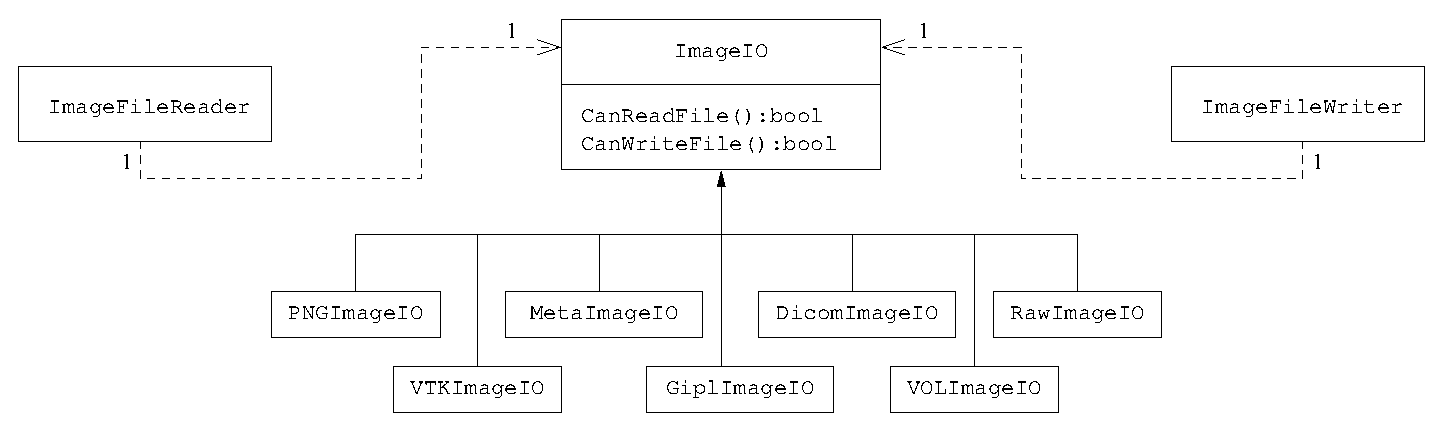
\includegraphics[width=\textwidth]{ImageIOCollaborationDiagram.eps}
\itkcaption[Collaboration diagram of the ImageIO classes]{Collaboration diagram
of the ImageIO classes.} \label{fig:ImageIOCollaborationDiagram}
\end{figure}

\begin{figure}
\center
\includegraphics[width=\textwidth]{ImageIOFactoriesUseCases.eps}
\itkcaption[Use cases of ImageIO factories] {Use cases of ImageIO factories.}
\label{fig:ImageIOFactoriesUseCases}
\end{figure}

\begin{figure}
\center
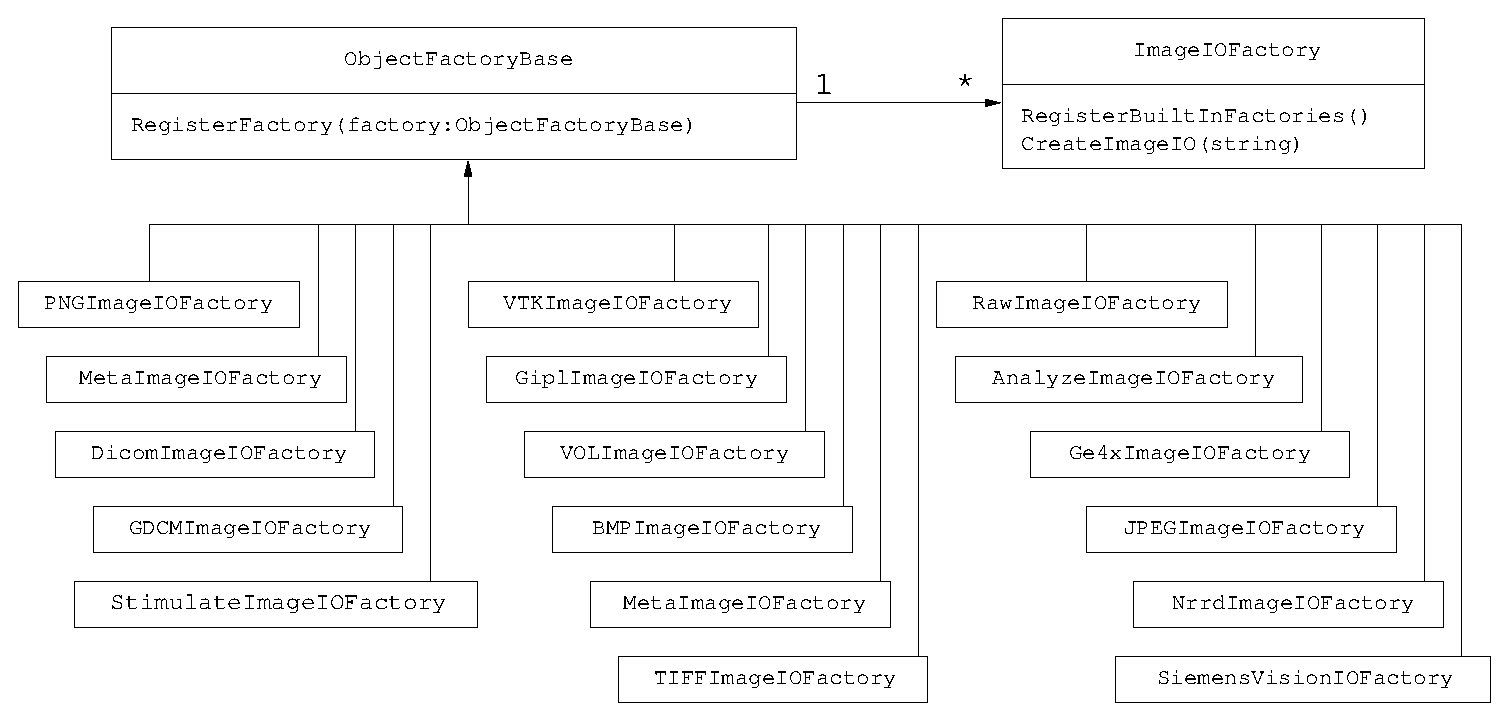
\includegraphics[width=\textwidth]{ImageIOFactoriesClassDiagram.eps}
\itkcaption[Class diagram of ImageIO factories] {Class diagram of the ImageIO
factories.}
\label{fig:ImageIOFactoriesClassDiagram}
\end{figure}

\section{Reading and Writing RGB Images}
\label{sec:RGBImagReadWrite}
\input{RGBImageReadWrite.tex}

\section{Reading, Casting and Writing Images}
\label{sec:ImagReadCastWrite}
\input{ImageReadCastWrite.tex}

\section{Extracting Regions}
\label{sec:ImagReadRegionOfInterestWrite}
\input{ImageReadRegionOfInterestWrite.tex}

\section{Extracting Slices}
\label{sec:ImagReadExtractWrite}
\input{ImageReadExtractWrite.tex}

\section{Reading and Writing Vector Images}
\label{sec:VectorImagReadWrite}

\input{CovariantVectorImageWrite.tex}

Let's now take the image that we just created and read it into another program.

\input{CovariantVectorImageRead.tex}


\section{Extracting Components from Vector Images}
\label{sec:VectorImageExtractComponent}
\input{CovariantVectorImageExtractComponent.tex}

\section{Reading Image Series}
\label{sec:ReadingImageSeries}
\input{ImageSeriesReadWrite.tex}
\input{RGBImageSeriesReadWrite.tex}


\section{Writing Image Series}
\label{sec:WritingImageSeries}
\input{ImageReadImageSeriesWrite.tex}

\section{Reading and Writing DICOM Images}
\label{sec:ReadingDicomImageSeries2}

% Small intro to DICOM file format

\subsection{Foreword}
ACR (the American College of Radiology) and NEMA (the National Electrical Manufacturers Association)
formed a joint committee to develop a Standard for Digital Imaging and COmmunications in Medicine (DICOM).
This DICOM Standard was developed according to the NEMA Procedures. This Standard is developed in liaison with other Standardization Organizations such as CEN TC251, JIRA including IEEE, HL7 and ANSI USA as reviewers.

With the introduction of computed tomography (CT) followed by other digital diagnostic imaging
modalities in the 1970's, and the increasing use of computers in clinical applications, the American
College of Radiology (ACR) and the National Electrical Manufacturers Association (NEMA) recognized
the emerging need for a standard method for transferring images and associated information between
devices manufactured by various vendors. These devices produce a variety of digital image formats.

DICOM is a comprehensive set of standards for handling, storing and transmitting information in medical
imaging. It includes both a file format definition as well as a network communication protocol.
DICOM was developed to enable integration of scanners, servers, workstations and network hardware from
multiple vendors into a picture archiving and communication system.

DICOM files consist of a header with standardized (See Insight/Utilities/gdcm/Dict/dicomV3.dic) as well 
as free-form fields and a body of image data. A single DICOM file can contain one or more frames, 
allowing storage of volumes or animations. Image data can be compressed using a variety of standards,
including JPEG, LZW and Run-length encoding (RLE).

The DICOM Standard is an evolving standard and it is maintained in accordance with the Procedures of
the DICOM Standards Committee. Proposals for enhancements are forthcoming from the DICOM
Committee member organizations based on input from users of the Standard. These proposals are
considered for inclusion in future editions of the Standard. A requirement in updating the Standard is to
maintain effective compatibility with previous editions. An entire newsgroup is dedicated to this: 
newsgroup://comp.protocols.dicom.

For a more detailed description of the DICOM standard see~\cite{DICOMStandard}.

\subsection{Reading and writing a 2D image}
\input{DicomImageReadWrite.tex}

\subsection{Reading a 2D DICOM Serie and writting a volume}
\input{DicomSeriesReadImageWrite2.tex}

\subsection{Reading a 2D DICOM serie and writting a 2D DICOM serie}
\input{DicomSeriesReadSeriesWrite.tex}



The following section describes the internals of the IO architecture provided
in the toolkit.

\section{Pluggable Factories}
\label{sec:ImageIOPluggableFactories}

The principle behind the input/output mechanism used in ITK is known as
\emph{pluggable-factories} \cite{Gamma1995}. This concept is illustrated in
the UML diagram in Figure~\ref{fig:ImageIOCollaborationDiagram}. From the
user's point of view the objects responsible for reading and writing files
are the \doxygen{ImageFileReader} and \doxygen{ImageFileWriter}
classes. These two classes, however, are not aware of the details involved in
reading or writing particular file formats like PNG or DICOM.  What they do
is to dispatch the user's requests to a set of specific classes that are
aware of the details of image file formats. These classes are the
\doxygen{ImageIO} classes. The ITK delegation mechanism enables users to
extend the number of supported file formats by just adding new classes to the
ImageIO hierarchy.

Each instance of ImageFileReader and ImageFileWriter has
a pointer to an ImageIO object. If this pointer is empty, it will
be impossible to read or write an image and the image file reader/writer must
determine which ImageIO class to use to perform IO operations.
This is done basically by passing the filename to a centralized class, the
\doxygen{ImageIOFactory} and asking it to identify any subclass of
ImageIO capable of reading or writing the user-specified file. This
is illustrated by the use cases on the right side of
Figure~\ref{fig:ImageIOFactoriesUseCases}.

Each class derived from ImageIO must provide an associated factory
class capable of producing an instance of the ImageIO class. For
example, for PNG files, there is a \doxygen{PNGImageIO} object that knows how
to read this image files and there is a \doxygen{PNGImageIOFactory} class
capable of constructing a PNGImageIO object and returning a pointer
to it.  Each time a new file format is added (i.e., a new ImageIO
subclass is created), a factory must be implemented as a derived class of the
ImageIOFactory class as illustrated in
Figure~\ref{fig:ImageIOFactoriesClassDiagram}.

For example, in order to read PNG files, a PNGImageIOFactory is
created and registered with the central ImageIOFactory
singleton\footnote{\emph{Singleton} means that there is only one instance of
this class in a particular application} class as illustrated in the left side
of Figure~\ref{fig:ImageIOFactoriesUseCases}. When the ImageFileReader asks
the ImageIOFactory for an ImageIO capable of reading the
file identified with \emph{filename} the ImageIOFactory will iterate over the
list of registered factories and will ask each one of them is they know how
to read the file. The factory that responds affirmatively will be used to
create the specific ImageIO instance that will be returned to the
ImageFileReader and used to perform the read operations.

In most cases the mechanism is transparent to the user who onlt interacts
with the ImageFileReader and ImageFileWriter. It is
possible, however, to explicitly select the type of ImageIO object
to use.  This is illustrated by the following example.


\section{Using ImageIO Classes Explicitly}
\label{sec:ImageReadExportVTK}
\input{ImageReadExportVTK.tex}




%%% \chapter{Numerics.tex}

Making use of the numerics libraries; interface classes to the numerics classes

\fi

\ifitkFullVersion
\chapter{Registration}

Examples of registration including an overview of the registration framework

\fi

\ifitkFullVersion

\chapter{Segmentation}

Segmentation of medical images is a challenging task. A myriad of
different methods have been proposed and implemented in recent
years. In spite of the huge effort invested in this problem, there is
no single approach that could generally solve the problem of
segmentation for the large variety of image modalities existing today.

The most effective segmentation algorithms are obtained by carefully
customizing combinations of components. The parameters of these components are
tuned for the characteristics of the image modality used as input and the
features of the anatomical structure to be segmented. 

The Insight toolkit provides a basic set of algorithms that can be used to
develop and customize a full segmentation application. Some of the most
commonly used segmentation components are described in the following sections.


\section{Region Growing}

Region growing algorithms have proven to be a very effective approach for image
segmentation. The basic concept of a region growing algorithm is to start from
a seed region that is considered to belong to the object to be segmented. The
pixels neigboring this initial region are evaluated to determine if they could
also be considered part of the object, in which case they are added to the
region. When some of the neighbor pixels are included in the region, other
pixels become new neighbors and hence become candidates to be evaluated and
eventually included in the region. Region growing algorithms vary depending on
the criteria used to decide whether a pixel should be included in the region
or not, the type of neighbor connectivity used on the image grid and the
strategy used for visiting the neighbor pixels.

Several implementations of region growing are available in the
Insight toolkit. This section describes some of the most commonly used.

\subsection{Connected Threshold}

The simplest criterion for including pixels in a growing region is
probably the condition of having intensity values inside a specific
interval.

\label{sec:ConnectedThreshold}
\ifitkFullVersion 
\input{ConnectedThresholdImageFilter.tex}
\fi


\subsection{Neighborhood Connected}
\label{sec:NeighborhoodConnectedImageFilter}
\ifitkFullVersion 
\input{NeighborhoodConnectedImageFilter.tex}
\fi



\subsection{Confidence Connected}
\label{sec:ConfidenceConnected}
\ifitkFullVersion 
\input{ConfidenceConnected.tex}
\fi


\subsection{Isolated Connected}
\label{sec:IsolatedConnected}
\ifitkFullVersion 
\input{IsolatedConnectedImageFilter.tex}
\fi


\section{Segmentation Based on Watersheds}
\label{sec:WatershedSegmentation}
\ifitkFullVersion 
\input WatershedSegmentation.tex
\fi


\section{Level Sets Segmentation}
\label{sec:LevelSetsSegmentation}
\ifitkFullVersion 
%%%%%%%%%%%%%%%%%%%%%%%%%%%%%%%%%%%%%%%%%%%%%%%%%%%%%%%%%%%%%%%%%%%%%%%%
%
%
%     This file is included from the file   Segmentation.tex
% 
%     Section tag and label are placed in this top file.
%
%
%
%%%%%%%%%%%%%%%%%%%%%%%%%%%%%%%%%%%%%%%%%%%%%%%%%%%%%%%%%%%%%%%%%%%%%%%%



\subsection{Threshold Level Set Segmentation}

\subsection{Fast Marching Segmentation}

\subsection{Shape Detection Segmentation}

\subsection{Geodesic Contours Segmentation}



\subsection{Segmentation Level Set Image Filter}
\label{sec:SegmentationLevelSetImageFilter}



\fi


\section{Hybrid Methods} 
\label{sec:HybridSegmentationMethods}

\ifitkFullVersion 
%%%%%%%%%%%%%%%%%%%%%%%%%%%%%%%%%%%%%%%%%%%%%%%%%%%%%%%%%%%%%%%%%%%%%%%%
%
%
%     This file is included from the file   Segmentation.tex
% 
%     Section tag and label are placed in this top file.
%
%
%
%%%%%%%%%%%%%%%%%%%%%%%%%%%%%%%%%%%%%%%%%%%%%%%%%%%%%%%%%%%%%%%%%%%%%%%%

\subsection{Introduction}
\label{sec:HybridSegmentationIntroduction}


It is sometimes convenient to combine several segmentation strategies with the
aim of taking advantage of their qualities an compensate their vulnerabilities.
The synergy between fundamentally different methodologies tends to result in
robustness and higher segmentation quality.  This section illustrates an hybrid
approach for segmentation in which two different strategies are configured to
work together. In this case, an input image is first processed by a filter
based on the concept of region growing. The criterion of acceptance in the
region is defined by a similarity measure that evaluates how homogeneous is the
path between to pixels. The output of this filter is used as a prior for
another filter that performs a full partition of the image space and then work
joining and splitting regions in order to optimize an homogeneity measure.
Details on the concepts behind those methods have been discussed in the
litterature
\cite{Angelini2002,Udupa2002,Jin2002,Imielinska2001,Imielinska2000a,Imielinska2000b}



\subsection{Background}
\label{sec:HybridSegmentationBackground}




%%%%%%%%%%%%%%%%%%%%%%%%%%%%%%%%%%%%%%%%%%%%%%%%%%%%%%%%%%%%%%%%%
%
%  Here is an example of how to include diagram in a figure
%
%  The file HybridSegmentationDiagram1.fig should be in the "Art"
%  directory. CMake will convert it to EPS before running latex. 
%
%%%%%%%%%%%%%%%%%%%%%%%%%%%%%%%%%%%%%%%%%%%%%%%%%%%%%%%%%%%%%%%%%

\begin{figure}
\center
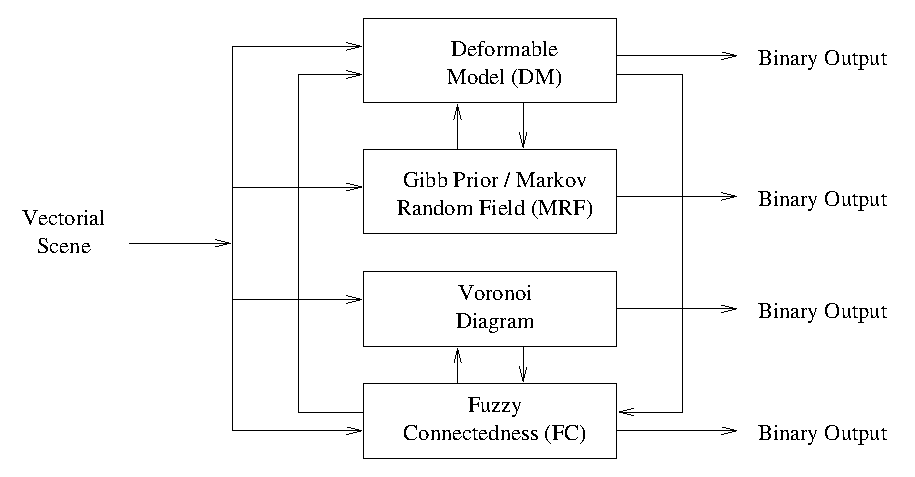
\includegraphics[width=6cm]{HybridSegmentationEngine1.eps}
\caption{Components of a HybridSegmentation approach}
\label{fig:HybridSegmentationEngine1}
\end{figure}

The Figure \ref{fig:HybridSegmentationEngine1} illustrates the main
components of the hybrid segmentation algorithm.

\begin{figure}
\center
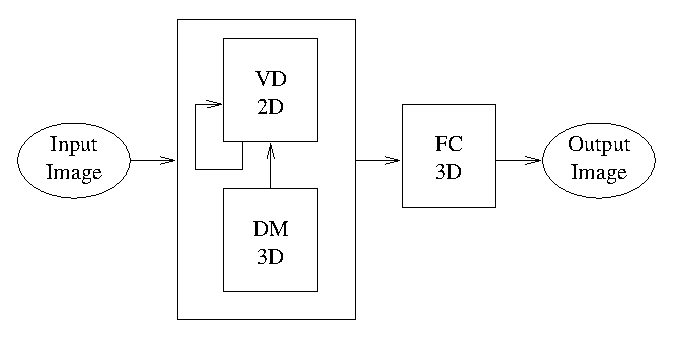
\includegraphics[width=6cm]{HybridSegmentationFCVDDM.eps}
\caption{Components of a HybridSegmentation approach}
\label{fig:HybridSegmentationFCVDDM}
\end{figure}


\begin{figure}
\center
\includegraphics[width=6cm]{VoronoiSegmentationClassDiagram1.eps}
\caption{UML Class Diagram of the VoronoiSegmentation filter}
\label{fig:VoronoiSegmentationClassDiagram1}
\end{figure}


\begin{figure}
\center
\includegraphics[width=6cm]{FuzzyConnectednessClassDiagram1.eps}
\caption{UML Class Diagram of the FuzzyConnectedness filter}
\label{fig:FuzzyConnectednessClassDiagram1}
\end{figure}


\begin{figure}
\center
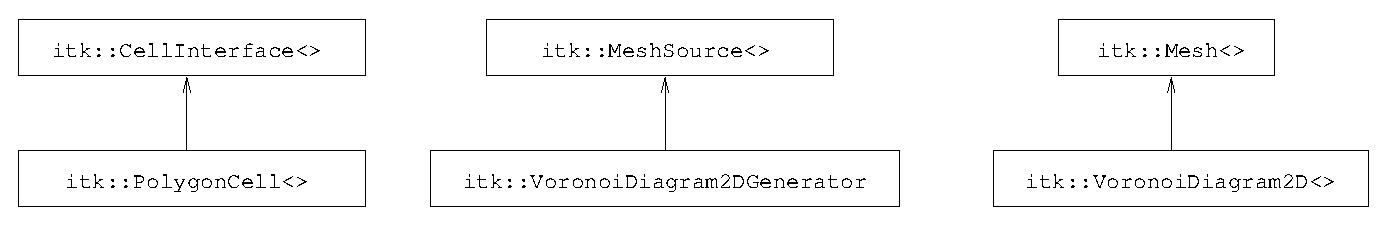
\includegraphics[width=6cm]{VoronoiSegmentationCollaborationDiagram1.eps}
\caption{UML Collaboration Diagram of the VoronoiSegmentation filter}
\label{fig:VoronoiSegmentationCollaborationDiagram1}
\end{figure}



\begin{figure}
\center
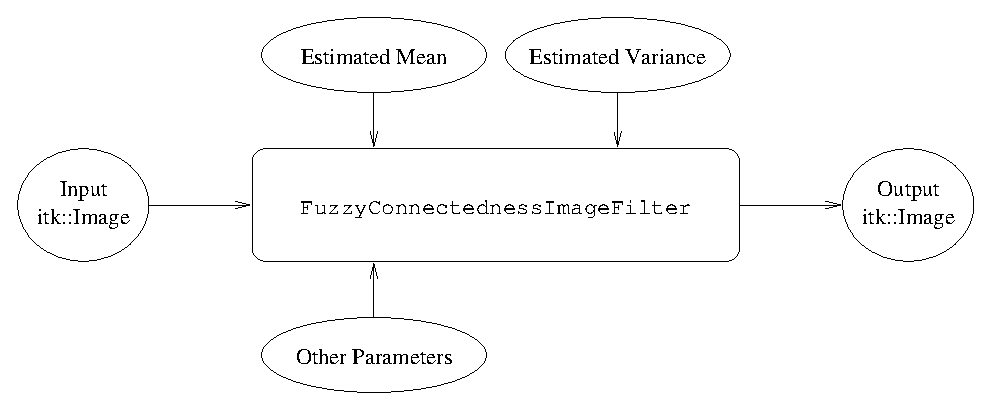
\includegraphics[width=6cm]{FuzzyConnectednessCollaborationDiagram1.eps}
\caption{UML Collaboration Diagram of the FuzzyConnectedness filter}
\label{fig:FuzzyConnectednessCollaborationDiagram1}
\end{figure}



\begin{figure}
\center
\includegraphics[width=6cm]{VoronoiSegmentationCollaborationDiagram2.eps}
\caption{UML Collaboration Diagram of the VoronoiSegmentation filter}
\label{fig:VoronoiSegmentationCollaborationDiagram2}
\end{figure}




\begin{figure}
\center
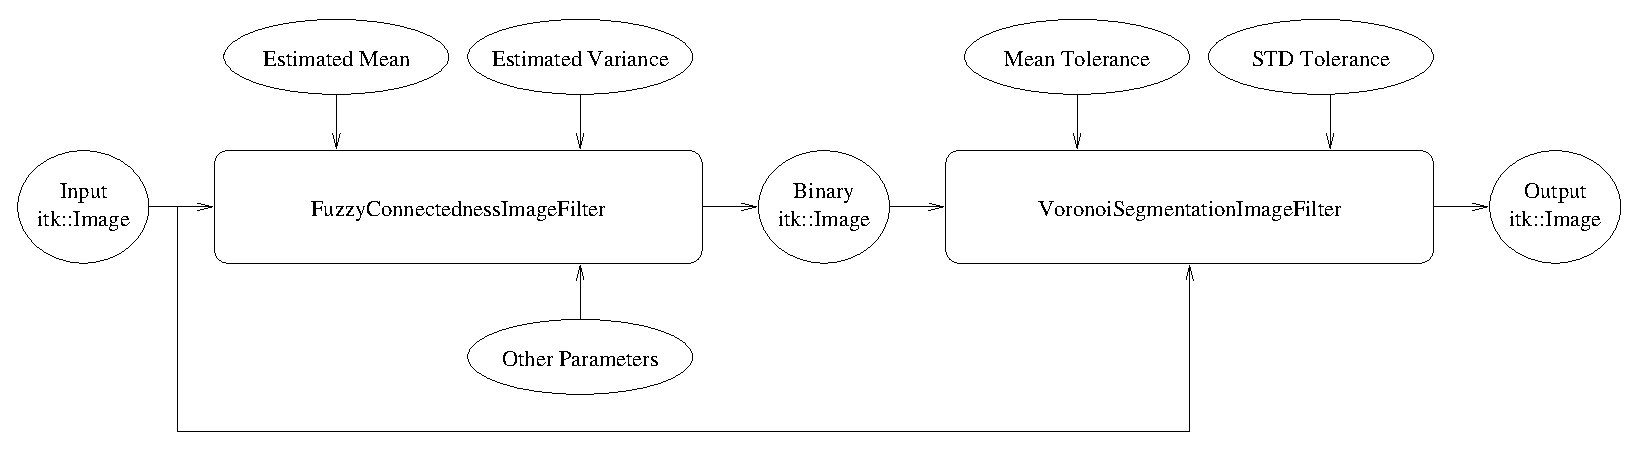
\includegraphics[width=6cm]{FuzzyVoronoiCollaborationDiagram1.eps}
\caption{UML Collaboration Diagram of the Fuzzy Voronoi Segmentation}
\label{fig:FuzzyVoronoiCollaborationDiagram1}
\end{figure}




\begin{figure}
\center
\includegraphics[width=6cm]{FuzzyVoronoiDeformableCollaborationDiagram1.eps}
\caption{UML Collaboration Diagram of the Fuzzy Voronoi Deformable Segmentation}
\label{fig:FuzzyVoronoiDeformableCollaborationDiagram1}
\end{figure}









%%%%%%%%%%%%%%%%%%%%%%%%%%%%%%%%%%%%%%%%%%%%%%%%%%%%%%%%%%%%%%%%%
%
%  Here is an example of how to include equations
%
%%%%%%%%%%%%%%%%%%%%%%%%%%%%%%%%%%%%%%%%%%%%%%%%%%%%%%%%%%%%%%%%%


\begin{equation}
MS(A,B) = \frac{1}{N} \sum_i^N \left( A_i - B_i \right)^2
\end{equation}





\subsection{Example}
\label{sec:HybridSegmentationExample1}

\input{HybridSegmentationFuzzyVoronoi.tex}



\fi



\fi

\ifitkFullVersion
\chapter{Statistics}
\label{sec:StaisticsFramework}

This chapter introduces the statistics functionalities in Insight. The
statistics subsystem's primary purpose is to provide general capabilities
for statistical pattern classification. However, its use is not limited
for classification. Users might want to use data containers and
algorithms in the statistics subsystem to perform other statistical
analysis or to preprocessor image data for other tasks.

The statistics subsystem mainly consists of three parts: data container
classes, statistical algorithms, and the classification framework. In this
chapter, we will discuss each major part in that order.

\section{Data Containers}
\label{sec:StatisticsDataContainer}

An \subdoxygen{Statistics}{Sample} object is a data container of elements
that we call \emph{measurement vectors}. A measurement vector is an array of
values (of the same type) measured on an object (In images, it can be a
vector of the gray intensity value and/or the gradient value of a
pixel). Strictly speaking from the design of the Sample class, a measurement
vector can be any class derived from \doxygen{FixedArray}, including
FixedArray itself.

\begin{figure}
  \centering
  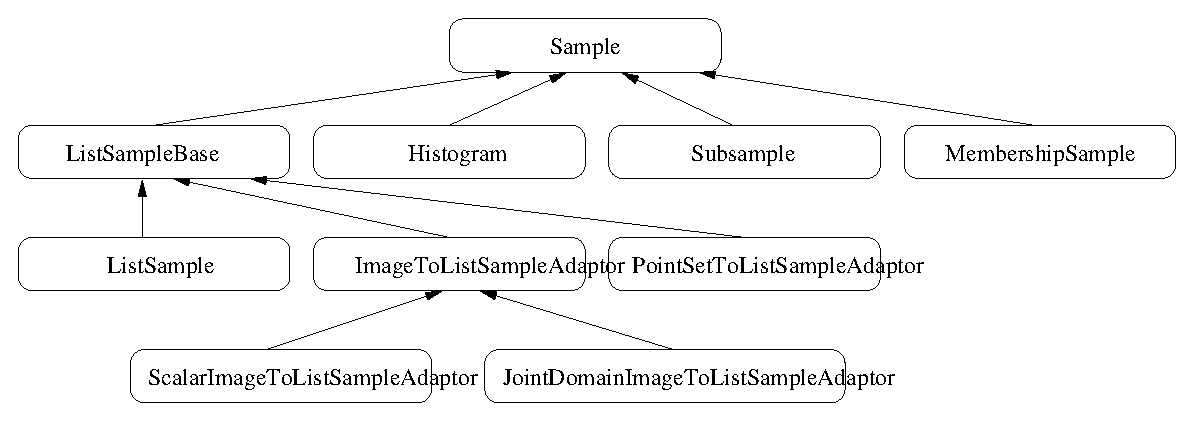
\includegraphics[width=0.9\textwidth]{SampleInheritanceTree.eps}
  \itkcaption[Sample class inheritance tree]{Sample class inheritance diagram.}
  \protect\label{fig:SampleInheritanceTree}
\end{figure}

\subsection{Sample Interface}
\label{sec:SampleInterface}

\ifitkFullVersion 
\input{ListSample.tex}
\fi

\subsection{Sample Adaptors}
\label{sec:SampleAdaptors}

There are two adaptor classes that provide the common
\subdoxygen{Statistics}{Sample} interfaces for \doxygen{Image} and
\doxygen{PointSet}, two fundamental data container classes found in ITK. The
adaptor classes do not store any real data elements themselves. These data
comes from the source data container plugged into them. First, we will
describe how to create an
\subdoxygen{Statistics}{ImageToListAdaptor} and then an
\subdoxygen{statistics}{PointSetToListAdaptor} object.

\subsubsection{ImageToListAdaptor}
\label{sec:ImageToListAdaptor}

\ifitkFullVersion 
\input{ImageToListAdaptor.tex}
\fi

\subsubsection{PointSetToListAdaptor}
\label{sec:PointSetToListAdaptor}

\ifitkFullVersion 
\input{PointSetToListAdaptor.tex}
\fi

\ifitkFullVersion 
\input{PointSetToAdaptor.tex}
\fi


\subsection{Histogram}
\label{sec:Histogram}

\ifitkFullVersion 
\input{Histogram.tex}
\fi

\subsection{Subsample}
\label{sec:Subsample}

\ifitkFullVersion 
\input{Subsample.tex}
\fi

\subsection{MembershipSample}
\label{sec:MembershipSample}

\ifitkFullVersion 
\input{MembershipSample.tex}
\fi

\subsection{MembershipSampleGenerator}
\label{sec:MembershipSampleGenerator}

\ifitkFullVersion 
\input{MembershipSampleGenerator.tex}
\fi


\subsection{K-d Tree}
\label{sec:KdTree}

\ifitkFullVersion 
\input{KdTree.tex}
\fi

\section{Algorithms and Functions}
\label{sec:StatisticsAlgorithmsFunctions}

In the previous section, we described the data containers in the ITK
statistics subsystem. We also need data processing algorithms and statistical
functions to conduct statistical analysis or statistical classification using
these containers. Here we define an algorithm to be an operation over a set
of measurement vectors in a sample. A function is an operation over
individual measurement vectors. For example, if we implement a class
(\subdoxygen{Statistics}{EuclideanDistance}) to calculate the Euclidean
distance between two measurement vectors, we call it a function, while if we
implemented a class (\subdoxygen{Statistics}{MeanCalculator}) to calculate
the mean of a sample, we call it an algorithm.

\subsection{Sample Statistics}
\label{sec:SampleStatistics}

We will show how to get sample statistics such as means and covariance from
the (\subdoxygen{Statistics}{Sample}) classes. Statistics can tells us
characteristics of a sample. Such sample statistics are very important for
statistical classification. When we know the form of the sample distributions
and their parameters (statistics), we can conduct Bayesian classification. In
ITK, sample mean and covariance calculation algorithms are implemented. Each
algorithm also has its weighted version (see Section
\ref{sec:WeightedMeanCovariance}). The weighted versions are used in the
expectation-maximization parameter estimation process.

\subsubsection{Mean and Covariance}
\label{sec:MeanCovariance}

\ifitkFullVersion 
\input{SampleStatistics.tex}
\fi

\subsubsection{Weighted Mean and Covariance}
\label{sec:WeightedMeanCovariance}

\ifitkFullVersion 
\input{WeightedSampleStatistics.tex}
\fi

\subsection{Sample Generation}
\label{sec:SampleGeneration}

\subsubsection{ListSampleToHistogramFilter}
\label{sec:ListSampleToHistogramFilter}

\ifitkFullVersion 
\input{ListSampleToHistogramFilter.tex}
\fi

\subsubsection{ListSampleToHistogramGenerator}
\label{sec:ListSampleToHistogramGenerator}

\ifitkFullVersion 
\input{ListSampleToHistogramGenerator.tex}
\fi

\subsubsection{NeighborhoodSampler}
\label{sec:NeighborhoodSampler}

\ifitkFullVersion 
\input{NeighborhoodSampler.tex}
\fi

\subsubsection{SampleToHistogramProjectionFilter}
\label{sec:SampleToHistogramProjectionFilter}

\ifitkFullVersion 
\input{SampleToHistogramProjectionFilter.tex}
\fi




\subsection{Sample Sorting}
\label{sec:SampleSorting}

\ifitkFullVersion 
\input{SampleSorting.tex}
\fi

\subsection{Probability Density Functions}
\label{sec:ProbabilityDensityFunctions}

The probability density function (PDF) for a specific distribution returns
the probability density for a measurement vector. To get the probability
density from a PDF, we use the \code{Evaluate(input)} method. PDFs for
different distributions require different sets of distribution
parameters. Before calling the \code{Evaluate()} method, make sure to set the
proper values for the distribution parameters.

\subsubsection{Gaussian Distribution}
\label{sec:GaussianDensityFunction}

\ifitkFullVersion 
\input{GaussianDensityFunction.tex}
\fi

\subsection{Distance Metric}
\label{sec:DistanceMetric}

\subsubsection{Euclidean Distance}
\label{sec:EuclideanDistance}

\ifitkFullVersion 
\input{EuclideanDistance.tex}
\fi

\subsection{Decision Rules}
\label{sec:DecisionRules}

A decision rule is a function that returns the index of one data element in a
vector of data elements. The index returned depends on the internal logic of
each decision rule. The decision rule is an essential part of the ITK
statistical classification framework. The scores from a set of membership
functions (e.g. probability density functions, distance metrics) are compared
by a decision rule and a class label is assigned based on the output of the
decision rule. The common interface is very simple. Any decision rule class
must implement the \code{Evaluate()} method. In addition to this method,
certain decision rule class can have additional method that accepts prior
knowledge about the decision task. The
\doxygen{MaximumRatioDecisionRule} is an example of such a class.

The argument type for the \code{Evaluate()} method is
\code{std::vector< double >}. The decision rule classes are part of the
\code{itk} namespace instead of \code{itk::Statistics} namespace.

For a project that uses a decision rule, it must link the \code{itkCommon}
library. Decision rules are not templated classes.

\subsubsection{Maximum Decision Rule}
\label{sec:MaximumDecisionRule}

\ifitkFullVersion 
\input{MaximumDecisionRule.tex}
\fi

\subsubsection{Minimum Decision Rule}
\label{sec:MinimumDecisionRule}

\ifitkFullVersion 
\input{MinimumDecisionRule.tex}
\fi

\subsubsection{Maximum Ratio Decision Rule}
\label{sec:MaximumRatioDecisionRule}

\input{MaximumRatioDecisionRule.tex}

\subsection{Random Variable Generation}
\label{sec:RandomVariableGeneration}

A random variable generation class returns a variate when the
\code{GetVariate()} method is called. When we repeatedly call the method
for ``enough'' times, the set of variates we will get follows
the distribution form of the random variable generation class.
 
\subsubsection{Normal (Gaussian) Distribution}
\label{sec:NormalVariateGeneration}

\ifitkFullVersion 
\input{NormalVariateGenerator.tex}
\fi


\section{Statistics applied to Images}
\label{sec:StatisticsAppliedToImages}

\subsection{Image Histograms}
\label{sec:ImageHistogram}


\subsubsection{Scalar Image Histogram with Adaptor}
\label{sec:ScalarImageHistogramAdaptor}
\ifitkFullVersion 
\input{ImageHistogram1.tex}
\fi


\subsubsection{Scalar Image Histogram with Generator}
\label{sec:ScalarImageHistogramGenerator}
\ifitkFullVersion 
\input{ImageHistogram2.tex}
\fi


\subsubsection{Color Image Histogram with Generator}
\label{sec:ColorImageHistogramGenerator}
\ifitkFullVersion 
\input{ImageHistogram3.tex}
\fi


\subsubsection{Color Image Histogram Writing}
\label{sec:ColorImageHistogramGeneratorWriting}
\ifitkFullVersion 
\input{ImageHistogram4.tex}
\fi


\subsection{Image Information Theory}
\label{sec:ComputingImageEntropy}

Many concepts from Information Theory have been used successfully in the domain
of image processing. This section introduces some of such concepts and
illustrates how the statistical framework in ITK can be used for computing
measures that have some relevance in terms of Information Theory
\cite{Shannon1948,Shannon1949,Kullback1997}.


\subsubsection{Computing Image Entropy}
\label{sec:ComputingImageEntropy}

\index{Entropy!What's wrong in images}

The concept of Entropy has been introduced into image processing as a crude
mapping from its application in Communications. The notions of Information
Theory can be decepting and misleading when applied to images because their
language from Communication Theory does not necessarily maps to what people in
the Imaging Community use.

For example, it is commonly said that

\emph{``The Entropy of an image is a measure of the amount of information
contained in an image''}. 

This statement is fundamentally \textbf{incorrect}. 

The way the notion of Entropy is commonly measured in images is by first
assuming that the spatial location of a pixel in an image is irrelevant!  That
is, we simply take the statistical distribution of the pixel values as it can
be evaluated in a histogram and from that histogram we estimate the frequency
of the value associated to each bin. In other words, we simply assume that the
image is a set of pixels that are passing through a channel, just as things are
commonly considered for communication purposes.

Once the frequency of every pixel value has been estimated, Information Theory
defines that the amount of uncertainty that an observer will lose by taking one
pixel and finding its real value to be the one associated with the i-th bin of the
histogram, is given by $-\log_2{(p_i)}$, where $p_i$ is the frequency in that
histogram bin. Since a reduction in uncertainty is equivalent to an increase in
the amount of information in the observer, we conclude that measuring one pixel
and finding its level to be in the i-th bin results in an acquisition of
$-\log_2{(p_i)}$ bits of information\footnote{Note that \textbf{bit} is the unit of
amount of information. Our modern culture has vulgarized the bit and its
multiples, the Byte, KiloByte, MegaByte, GigaByte and so on as simple measures
of the amount of RAM memory and capacity of a hard drive in a computer. In that
sense, a confusion is created between the encoding of a piece of data and its
actual amount of information. For example a file composed of one million
letters will take one million bytes in a hard disk, but it does not necessariy
has one million bytes of information, since in many cases parts of the file can
be predicted from others. This is the reason why data compression can manage to
compact files.}.

Since we could have picked any pixel at random, our chances or picking the ones
that are associated to the i-th histogram bin are given by $p_i$. Therefore,
the expected reduction in uncertainty that we can get from measuring the value
of one pixel is given by

\begin{equation}
H = - \sum_i{ p_i  \cdot \log_2{(p_i)} }
\end{equation}

This quantity $H$ is what is usually defined as the \emph{Entropy of the
Image}. It would be more accurate to call it the Entropy of the random variable
associated to the intensity value of \emph{one} pixel. The fact that $H$ is
unrelated to the spatial arrangement of the pixels in an image shows how little
of the real \emph{Image Information} is $H$ actually representing. The Entropy
of an image, as mesure above, is only a crude indication of how the intensity
values are spread in the dynamic range of intensites. For example, an image
with maximum entropy will be the one that has a large dynamic range and every
value in that range is equally probable. 

The common acceptation of $H$ as a representation of image information has
terribly undermined the enormous potential on the application of Information
Theory to image processing and analysis.

The real concepts of Information Theory would require that we define the amount
of information in an image based on our expectations and prior knowledge from
that image. In particular, the \emph{Amount of Information} provided by an
image should measure the number of features that we are not able to predict
based on our prior knowledge about that image. For example, if we know that we
are going to analyze a CT scan of the abdomen of an adult human male in the age
range of 40 to 45, there is already a good deal that we could predict about the
content of that image.  The real amount of information in the image is the
representation of the features in the image that we could not predict from
knowing that it is a CT scan from a human adult male.

The application of Information Theory to image analysis is still in its early
infancy and it is an exciting an promising field to be explored further. All
that being said, let's now look closer at how the concept of Entropy (which is
not the amount of information in an image) can be measured with the ITK
statistics framework.

\ifitkFullVersion 
\input{ImageEntropy1.tex}
\fi

\subsubsection{Computing Images Mutual Information}
\label{sec:ComputingImagesMutualInformation}

\ifitkFullVersion 
\input{ImageMutualInformation1.tex}
\fi



\section{Classification}
\label{sec:Classification}

In statistical classification, each object is represented by $d$ features (a
measurement vector), and the goal of classification becomes finding compact and
disjoint regions (decision regions\cite{Duda2000}) for classes in a
$d$-dimensional feature space. Such decision regions are defined by decision
rules that are known or can be trained.  The simplest configuration of a
classification consists of a decision rule and multiple membership functions;
each membership function represents a class. Figure~\ref{fig:simple}
illustrates this general framework.

\begin{figure}[h]
  \centering
  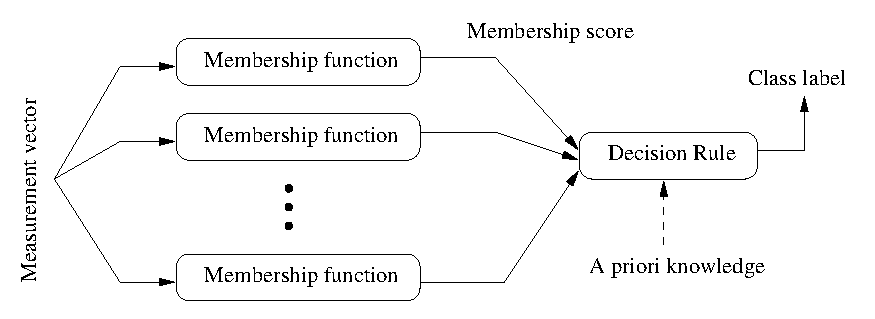
\includegraphics[width=0.7\textwidth]{DudaClassifier.eps}
  \itkcaption[Simple conceptual classifier]{Simple conceptual classifier.}
  \label{fig:simple}
\end{figure}

This framework closely follows that of Duda and
Hart\cite{Duda2000}. The classification process can be described
as follows:

\begin{enumerate}
\item{A measurement vector is input to each membership function.}
\item{Membership functions feed the membership scores to the
    decision rule.}
\item{A decision rule compares the membership scores and returns a
    class label.}
\end{enumerate}

\begin{figure}
  \centering
  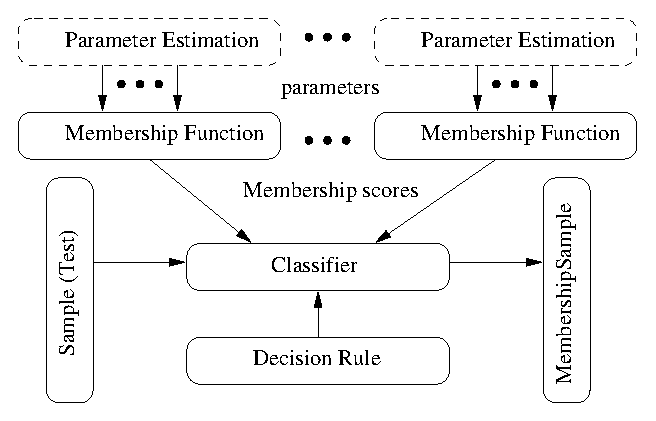
\includegraphics[width=0.7\textwidth]{StatisticalClassificationFramework.eps}
  \itkcaption[Statistical classification framework]{Statistical classification
framework.}
  \protect\label{fig:StatisticalClassificationFramework}
\end{figure}

This simple configuration can be used to formulated various classification
tasks by using different membership functions and incorporating task specific
requirements and prior knowledge into the decision rule. For example, instead
of using probability density functions as membership functions, through
distance functions and a minimum value decision rule (which assigns a class
from the distance function that returns the smallest value) users can achieve a
least squared error classifier. As another example, users can add a rejection
scheme to the decision rule so that even in a situation where the membership
scores suggest a ``winner'', a measurement vector can be flagged as ill
defined. Such a rejection scheme can avoid risks of assigning a class label
without a proper win margin.

\subsection{k-d Tree Based k-Means Clustering}
\label{sec:KdTreeBasedKMeansClustering}
\ifitkFullVersion
\input{KdTreeBasedKMeansClustering.tex}
\fi

\subsection{K-Means Classification}
\label{sec:KMeansClassifier}
\ifitkFullVersion
\input{ScalarImageKmeansClassifier.tex}
\fi

\subsection{Bayesian Plug-In Classifier}
\label{sec:BayesianPluginClassifier}

\ifitkFullVersion 
\input{BayesianPluginClassifier.tex}
\fi


\subsection{Expectation Maximization Mixture Model Estimation}
\label{sec:ExpectationMaximizationMixtureModelEstimation}

\ifitkFullVersion 
\input{ExpectationMaximizationMixtureModelEstimator.tex}
\fi

\subsection{Classification using Markov Random Field}
\label{sec:MarkovRandomField}

Markov Random Fields are probabilistic models that use the correlation between
pixels in a neighborhood to decide the object region. The
\subdoxygen{Statistics}{MRFImageFilter} uses the maximum a posteriori (MAP)
estimates for modeling the MRF. The object traverses the data set and uses the
model generated by the Mahalanobis distance classifier to gets the the distance
between each pixel in the data set to a set of known classes, updates the
distances by evaluating the influence of its neighboring pixels (based on a MRF
model) and finally, classifies each pixel to the class which has the minimum
distance to that pixel (taking the neighborhood influence under consideration).
The energy function minimization is done using the iterated coditional modes
(ICM) algorithm \cite{Besag1986}.

\ifitkFullVersion
\input{ScalarImageMarkovRandomField1.tex}
\fi 




\fi

%%% \chapter{Application}

Pointers and a brief description of the available ITK applications.




\ifitkFullVersion
\part{Developer's Guide}

%%% \chapter{Infrastructure}
\label{chapter:Infrastructure}

Smart pointers, exceptions, events, object factories

%%% \chapter{Iterators}

\index{Iterator!Concept}
\index{Generic Programming}
This chapter introduces the \emph{image iterator}, a fundamental and important
generic programming construct for image processing in ITK.  An iterator is a
generalization of the familiar C pointer, used to access data in memory.  ITK
has a wide variety of iterators, some of which are highly specialized to
simplify common image processing tasks.

The section that follows is a brief introduction that defines iterators in the
context of ITK and the \code{itk::Image} and describes their common programming
interface.  The specific types and instances of iterators are documented in the
last sections of this chapter, along with some examples of how they can be
used.

\section{Overview}
\label{sec:IteratorsIntroduction}
% Further define iterators in the context of generic programming.
Generic programming models define functionally independent components called
\emph{containers} and \emph{algorithms}.  Algorithms operate on data
within containers to produce some result.  Iterators keep these two components
independent of one another by presenting the algorithm object with a generic
interface that it can use to fetch and store data in any container object.
Using iterators, algorithm code can be written that does not depend on any one
specific representation of data.

% Define iterators in the context of ITK generic programming. 
In ITK, we use the iterator concept to write image processing code that can be
instantiated and run on \code{itk::Image}s of any combination of pixel type,
dimensionality, and pixel container type (see itk::Image).
Figure~\ref{fig:ImageIterators} illustrates how image iterators form the glue
between ITK filters (algorithms) and different ITK image types (data
containers). A filter processes data in an image one pixel at a time.  The
\emph{iterator} is incremented at each \emph{iteration} of the inner processing
loop.

\begin{figure}
\centering
%\includegraphics[width=0.9\textwidth]{}
%figure with small graphic illustrating algorithm & iterators plus some simple pseudocode.
\caption[Image iterators in ITK]{Image iterators in ITK}
\protect\label{fig:ImageIterators}
\end{figure}

% List advantages: code size/reuse. increased performance over set/get in image, allow to ignore
% dimensionality. 
There are many advantages to using image iterators over direct pixel access
through \code{itk::Image::Set} and \code{itk::Image::Get} methods.  Code is more
compact and often generalizes automatically to higher dimensions, algorithms
run much faster, and many tasks such as multithreading, neighborhood image
processing, and working with non-rectilinear regions of interest are greatly
simplified.  These advantages will be illustrated in the sections to follow. 

%In fact, with iterators,
%algorithms often generalize to higher dimensions automatically.  Note how the
%code in figure~\ref{fig:ImageIterators} is equally correct for images of two,
%three, or even ten dimensions.  The alternative to using iterators in this
%example would be a set of nested \code{for} loops.  Such nested loops would
%also require knowing the size of the image.  


% Talk about extensions to iterator concept, iterating through nonrectilinear
% regions.  Encapsulating complex tasks such as managing pointers to pixel
% neighbors in ND.
%Image iterators can encapsulate much of the complexity of writing many common
%algorithms.  Some ITK iterators, for example, have been designed to walk
%non-rectilinear paths through an image, allowing specialized processing over
%regions of interest or boundary pixels.  Other iterators efficiently manage
%access to entire N-dimensional neighborhoods, making localized image processing
%algorithms simple to write and to generalize to higher dimensions.


[describe a standard ITK interface]
Most ITK iterators define the following methods. [a bulleted definition list?]
        GoToBegin()
        GoToEnd()
        IsAtEnd()
        IsAtBegin()
        Operator++
        Operator--

[where traditional iterators overload the * operator, in ITK we have chosen to
use Set Get]
        Get
        Set
Set methods are only defined in const iterators.
Some iterators also supply a Value() method to allow dereferencing and modifying a
pixel value in a single step.  For example: [give example of how if you wanted
to do something like *it++ you would have to write it as it.Set(it.Get() + 1),
whereas it.Value()++ saves one dereference]

[image adaptors]
The use of Set, Get also supports image adaptors (section reference?)

[three basic types of image iterators: single pixel access methods, single
pixel methods which walk special paths, neighborhood access methods,]

The following sections describe the various ITK image iterator types.

\section{Image Iterators}
\label{sec:ImageIterators}



\subsection{itk::ImageRegionIterator}
\label{sec:itkImageRegionIterator}
./Common/itkImageRegionConstIterator.h
./Common/itkImageRegionIterator.h
(./Common/itkImageConstIterator.h base class)
(./Common/itkImageIterator.h base class)

Describe typical use cases.

Describe any special peculiarities of the interface and the guarantees of
complexity, etc.  Guarantees: will walk a region in same order on two different
images, no guarantees of what that order will be necessarily.

Example code

\subsection{itk::ImageRegionIteratorWithIndex}
\label{sec:itkImageRegionIteratorWithIndex}
./Common/itkImageRegionConstIteratorWithIndex.h
./Common/itkImageRegionIteratorWithIndex.h
(./Common/itkImageConstIteratorWithIndex.h  base class )
(./Common/itkImageIteratorWithIndex.h  base class )

\subsection{itk::ImageSliceIteratorWithIndex}
\label{sec:itkImageSliceIteratorWithIndex}
./Common/itkImageSliceConstIteratorWithIndex.
./Common/itkImageSliceIteratorWithIndex.h

\subsection{itk::ImageLinearIteratorWithIndex}
\label{sec:itkImageLinearIteratorWithIndex}
./Common/itkImageLinearConstIteratorWithIndex.h
./Common/itkImageLinearIteratorWithIndex.h

\subsection{itk::ImageRandomConstIteratorWithIndex}
\label{sec:itkImageRandomConstIteratorWithIndex}
./Common/itkImageRandomConstIteratorWithIndex.h
./Common/itkImageRandomIteratorWithIndex.h


\section{Conditional Iterators}
\label{sec:ConditionalIterators}

[Introduction and overview]

./Common/itkConditionalConstIterator.h (BaseClass)
./Common/itkConditionalIterator.h (BaseClass)
./Common/itkFloodFilledFunctionConditionalConstIterator.h (BaseClass)
./Common/itkFloodFilledFunctionConditionalIterator.h (BaseClass)


%[ here are all classes where these filters are used:
% ./BasicFilters/itkConfidenceConnectedImageFilter.txx (ImageFunction)
% ./BasicFilters/itkConnectedThresholdImageFilter.txx (ImageFunction)
% ./BasicFilters/itkIsolatedConnectedImageFilter.txx (ImageFunction)
% ./BasicFilters/itkNeighborhoodConnectedImageFilter.txx (ImageFunction)
%
% ./Common/itkBinaryBallStructuringElement.txx (SpatialFunction)
% ./Common/itkBloxCoreAtomImage.txx (SpatialFunction)
% ./BasicFilters/itkBloxBoundaryPointToCoreAtomImageFilter.txx (SpatialFunction)
% ./BasicFilters/itkBloxBoundaryPointImageToBloxBoundaryProfileImageFilter.txx (SpatialFunction)
%]

\subsection{itk::FloodFilledImageFunctionConditionalIterator}
\label{itk::FloodFilledImageFunctionConditionalIterator}
./Common/itkFloodFilledImageFunctionConditionalConstIterator.h
./Common/itkFloodFilledImageFunctionConditionalIterator.h


\subsection{itk::FloodFilledSpatialFunctionConditionalIterator}
\label{itk::FloodFilledSpatialFunctionConditionalIterator}
./Common/itkFloodFilledSpatialFunctionConditionalConstIterator.h
./Common/itkFloodFilledSpatialFunctionConditionalIterator.h


\section{Neighborhood Iterators}
\label{sec:NeighborhoodIterators}

[Introduction goes here]
[Be sure to reference Section: Neighborhood Filters]

% Example: derivative
% Example: convolution filtering
% Example: boundary conditions
% Example: walking faces

\subsection{itk::NeighborhoodIterator}
\label{sec:itkNeighborhoodIterator}
./Common/itkConstNeighborhoodIterator.h
./Common/itkNeighborhoodIterator.h

\subsection{itk::ShapedNeighborhoodIterator}
\label{sec:itkShapedNeighborhoodIterator}
./Common/itkConstShapedNeighborhoodIterator.h
./Common/itkShapedNeighborhoodIterator.h























\input{WriteAFilter.tex}
%%% \chapter{GUI}

Interface to GUI's such as FLTK, Qt, and wxWindows

%%% \chapter{Wrapping}

Using wrappers and generating wrappers.


\chapter{Software Process}
\label{chapter:SoftwareProcess}

An outstanding feature of ITK is the software process used to develop,
maintain, and test the toolkit. The Insight Toolkit software continues
to evolve rapidly due to the efforts of developers and users located around
the world, so the software process is essential to maintaining its
quality. If you are planning to contribute to ITK, or use the CVS source code
repository or the daily releases, you need to know something about this
process (see \ref{sec:ObtainingTheSoftware} on page 
\pageref{sec:ObtainingTheSoftware} to learn more about 
obtaining ITK using CVS). This information will help you know when and how to
update and work with the software as it changes. The following sections
describe key elements of the process.

\section{CVS Source Code Repository}
\label{sec:CVSRepository}

\index{ITK!CVS repository}
\index{CVS|textbf}

The Concurrent Versions System (CVS) is a tool for version control
\cite{Fogel1999}. It is a very valuable resource for software projects
involving multiple developers.  The primary purpose of CVS is to keep track
of changes to software. CVS date and version stamps every addition to the
repository---also providing for special user-specified tags---so that it is
possible to return to a particular state or point of time whenever
desired. The differences between any two points is represented by a ``diff''
file, that is a compact, incremental representation of change. CVS supports
concurrent development so that two developers can edit the same file at the
same time, that are then (usually) merged together without incident (and
marked if there is a conflict). In addition, branches off of the main
development trunk provide parallel development of software.

Developers and users can check out the software from the CVS repository. When
developers introduce changes in the system,  CVS facilitates to update the
local copies of other developers and users by downloading only the differences
between their local copy and the version on the repository.  This is an
important advantage for those who are interested in keeping up to date with the
leading edge of the toolkit. Bug fixes can be obtained in this way as soon as
they have been checked into the system.

ITK source code, data, and examples are maintained in a CVS repository.
The principal advantage of a system like CVS is that it frees developers to
try new ideas and changes without fear of losing a previous working version
of the software. It also provides a simple way to incrementally update code
as new features are added to the repository.



\section{DART Regression Testing System}
\label{sec:DART}
\label{sec:QualityDashboard}

\index{Dashboard|textbf}
\index{Quality Dashboard|textbf}
\index{Dart|textbf}

One of the unique features of the ITK software process is its use of the DART
regression testing system (\url{http://public.kitware.com/Dart}). In a
nutshell, what DART does is to provide quantifiable feedback to developers as
they check in new code and make changes. The feedback consists of the results
of a variety of tests, and the results are posted on a publically-accessible
Web page (to which we refer as a \emph{dashboard} as shown in Figure
\ref{fig:Dashboard} and accessible from
\url{http://www.itk.org/Testing/Dashboard/MostRecentResults-Nightly/Dashboard.html}).
All users and developers of ITK can view the dashboard, that produces
considerable peer-pressure on developers who check in code with problems. The
Dart dashboard serves as the vehicle for developer communication, and should
be viewed whenever you consider updating software via CVS or a daily release.

\begin{figure}[ht]
\centering 
\includegraphics[width=0.7\textwidth]{Dashboard.eps}
\itkcaption[Dart Quality Dashboard]{On-line presentation of the Quality
Dashboard generated by Dart}
\label{fig:Dashboard}
\end{figure}

Note that DART is independent of ITK and can be used to manage quality
control for any software project. It is itself an open-source package and can
be obtained from

\begin{center} 
\url{http://public.kitware.com/Dart/HTML/Index.shtml}
\end{center} 

DART supports a variety of test types. These include the following.
\begin{description}
        \item[Compilation.] All source code is compiled and linked. Any
        resulting errors and warnings are reported.

        \item[Regression.] Most ITK tests produce images as output. Testing
        requires comparing each test�s output against a valid image. If
        the images match then the test passes. The comparison must be
        performed carefully since many 3D graphics systems (e.g., OpenGL)
        produce slightly different results on different platforms.

        \item[Memory.] One of the nastiest of problems to find in any
        computer program are those related to memory. Memory leakage,
        uninitialized memory, and reads and writes beyond allocated space are
        all examples of this sort of problem. ITK checks memory using Purify,
        a commercial package produced by Rational. (Other memory checking
        programs will be added in the future.)

        \item[PrintSelf.] All classes in ITK are expected to print out all
        their instance variables correctly. This test checks to make sure
        that this is the case.

        \item[SetGet.] Often developers make assumptions about the values of
        instance variables; i.e., they assume that they are non-NULL,
        etc. The SetGet tests perform a Get on all instance variables with a
        Get\_\_() method, followed by a Set method on the instance variable
        with the value returned from the Get\_\_() method. It's surprising
        how many times this test identifies problems.

        \item[TestEmptyInput.] This deceptively simple test catches many
        problems due to developers assuming that the input to a process
        object is non-NULL, or that the input data object contains some
        data. TestEmptyInput simply exercises these two conditions on each
        subclass of vtkProcessObject and reports problems if encountered.

        \item[Coverage.] There is a saying among ITK developers: \emph{If it
        isn't covered, then it's broke.} What this means is that
        code that is not executed during testing is likely to be wrong. The
        coverage tests identify lines that are not executed in the
        Insight Toolkit test suite, reporting a total percentage
        covered at the end of the test. While it is nearly impossible to
        bring the coverage to 100\% because of error handling code and similar
        constructs that are rarely encountered in practice, the coverage
        numbers should be 75\% or higher. Code that is not covered well enough
        requires additional tests.
\end{description}

Figure \ref{fig:Dashboard} shows the top-level Dashboard Web page. Each row
in the Dashboard corresponds to a particular platform (hardware + operating
system + compiler). The data on the row indicates the number of compile
errors and warnings as well as the results of running hundreds of
small test programs. In this way the toolkit is tested both at compile time
and run time.

When users decide to download a daily release or a CVS version of ITK it is
important for them to verify first that the current dashboard is in good
shape. This can be rapidly judged by the general coloration of the
dashboard. A green state means that the software is building correctly and it
is a good day to start with ITK or to get an upgrade. A red state, on the
other hand, is an indication of instability on the system and hence users
should better refrain from checking out or upgrading.

Another nice feature of DART is that it maintains a history of changes to the
source code (by coordinating with CVS) and summarizes the changes as part of
the dashboard. This is useful for tracking problems and keeping up to date
with new additions to ITK.

\section{Working The Process}
\label{sec:WorkingTheProcess}

The ITK software process functions across three cycles---the continuous
cycle, the daily cycle, and the release cycle.

The continuous cycle revolves around the actions of developers as they check
code into CVS. When changed or new code is checked into CVS, the DART
continuous testing process kicks in. A small number of tests are performed
(including compilation), and if something breaks, email is sent to all
developers who checked code in during the continuous cycle. Developers are
expected to fix the problem immediately.

The daily cycle occurs over a 24-hour period. Changes to the source base made
during the day are extensively tested by the nightly DART regression testing
sequence. These tests occur on different combinations of computers and
operating systems located around the world, and the results are posted every
day to the DART dashboard. Developers who checked in code are expected to
visit the dashboard and ensure their changes are acceptable---that is, they
do not introduce compilation errors or warnings, or break any other tests
including regression, memory, print self, and Set/Get. Developers are
expected to fix problems immediately.

The release cycle occurs a small number of times a year. This requires
tagging and branching the CVS repository, updating documentation, and
producing new release packages. Although additional testing is performed to
insure the consistency of the package, keeping the daily releases error free
minimizes the work required to cut a release.

ITK users typically work with releases, since they are the most
stable. Developers work with the CVS repository, or sometimes with periodic
snapshots (a particular daily release) in order to take advantage of a
newly-added feature. It is extremely important that developers watch the
dashboard carefully, and \emph{update their software (via CVS or a new daily
release install) only when the dashboard is in good condition (i.e., is
``green'')}. Failure to do so can cause significant disruption if a
particular day's software release is unstable.

\section{The Effectiveness of the Process}
\label{sec:Effectiveness}

The effectiveness of this process is profound. By providing immediate
feedback to developers through email and Web pages (e.g., the dashboard), the
quality of ITK is exceptionally high, especially considering the complexity
of the algorithms and system. Errors, when accidently introduced, are caught
quickly, as compared to catching them at the point of release. To wait to the
point of release is to wait too long, since the causal relationship between a
code change or addition and a bug is lost. The process is so powerful that it
routinely catches errors in vendor's graphics drivers (e.g., OpenGL drivers)
or changes to external subsystems such as the Mesa OpenGL software
library. All of these tools that make up the process (CMake, CVS, and DART
are open-source). Many large and small systems such as VTK (The Visualization
Toolkit \url{http://www.vtk.org}) use the same process with similar
results. We encourage the adoption of the process in your environment.


\fi

\backmatter


%%%%%%%%%%%%%%%%%%%%%%%%%%%%%%%%%%%%%%%%%
%
% Insert List of Figures and Tables
%
%%%%%%%%%%%%%%%%%%%%%%%%%%%%%%%%%%%%%%%%%

\listoffigures
\listoftables


%%%%%%%%%%%%%%%%%%%%%%%%%%%%%%%%%%%%%%%%%
%
%  Insert the bibliography using BibTeX
%
%%%%%%%%%%%%%%%%%%%%%%%%%%%%%%%%%%%%%%%%%

\bibliographystyle{plain}
\bibliography{\bibtexdatabasepath}


%%%%%%%%%%%%%%%%%%%%%%%%%%%%%%%%%%%%%%%%%
%
%  Insert the Index file
%
%%%%%%%%%%%%%%%%%%%%%%%%%%%%%%%%%%%%%%%%%

\InputIfFileExists{SoftwareGuide.ind}



\end{document}



